\documentclass[12pt]{article} %%%%%%%%%%%%%%%%%%%%%%%%%%%
%%%%%%%%%%%%%%%%%%%%%%%%%%%%%%%%%%%%%%%%%%%%%%%%%%%%%%%%%
%%%
%%% Blank Sweave Document
%%%   This uses xelatex and MinionPro. Most users will need
%%%   to comment out stuff in the 'fonts' section below.
%%%   It should compile in regular pdflatex, if you comment
%%%   out xltxtra and fontspec.
%%% also, you probably need to comment out \usepackage{Sweave}
%%%   to allow R to insert its own ugly default one.
%%% 
%%% mjm / 2009-11-23 %%%%%%%%%%%%%%%%%%%%%%%%%%%%%%%%%%%%


%%% options to change font. If you want to play with MinionPro,
%%% come bug me sometime. --mike
%%% LOTS OF COOL FONT INFO AT http://www.tug.dk/FontCatalogue/
%%% NO NEED EVER TO USE COMPUTER MODERN, AN ABOMINATION
%%% see also http://nitens.org/taraborelli/latex and
%%% http://scripts.sil.org/XeTeX
%\usepackage{times}
%\usepackage{cmbright}
%\renewcommand\sfdefault{phv}% use helvetica for sans serif
%\renewcommand\familydefault{\sfdefault}% use sans serif by default
%\usepackage[dvipsnames,usenames]{xcolor}
%\usepackage[opticals,medfamily,minionint,footnotefigures]{MinionPro}
%\usepackage[no-math]{fontspec}
%\usepackage{xltxtra}



%%%Set up bold Minion Pro math
%\usepackage{bm}
%\DeclareMathAlphabet\mathbf {T1} {MinionPro-OsF}{b}{n}
%\SetMathAlphabet\mathit  {bold}{T1} {MinionPro-OsF}{b}{it}
%\SetSymbolFont{operators}{bold}{T1} {MinionPro-OsF}{b}{n}
%\SetSymbolFont{letters}  {bold}{OML}{MinionPro-TOsF} {b}{it}
%\DeclareMathVersion{boldtabular}
%\SetSymbolFont{operators}{boldtabular}{T1} {MinionPro-OsF}{b}{n}
%\SetSymbolFont{letters}  {boldtabular}{OML}{MinionPro-TOsF}  {b}{it}
%\SetMathAlphabet\mathit  {boldtabular}{T1} {MinionPro-OsF}{b}{it}
%\DeclareMathAlphabet\mathebf {T1} {MinionPro-OsF}{eb}{n}

%%% Hanging indents: args length, number of lines.
%%% \begin{hangparas}{1em}{1}
\usepackage{hanging} 
%%% Date formatting, defn of isodate
\usepackage{datetime}
\renewcommand{\dateseparator}{-}
\newdateformat{isodate}{%
\THEYEAR\dateseparator\twodigit{\THEMONTH}\dateseparator\twodigit{\THEDAY}}

%%% PDF setup -- fill in the title
%% Alter some LaTeX defaults for better treatment of figures:
%% This is from the first result of google: "latex dumb defaults"
    \renewcommand{\topfraction}{0.9}	
    \renewcommand{\bottomfraction}{0.8}	
    %   Parameters for TEXT pages (not float pages):
    \setcounter{topnumber}{2}
    \setcounter{bottomnumber}{2}
    \setcounter{totalnumber}{4}     
    \setcounter{dbltopnumber}{2}    
    \renewcommand{\dbltopfraction}{0.9}	
    \renewcommand{\textfraction}{0.07}	
    %   Parameters for FLOAT pages (not text pages):
    \renewcommand{\floatpagefraction}{0.7}	% require fuller float pages
	% N.B.: floatpagefraction MUST be less than topfraction !!
    \renewcommand{\dblfloatpagefraction}{0.7}	% require fuller float pages

%%% Enable the bibliography
%%%     see  http://merkel.zoneo.net/Latex/natbib.php
%%% 
%%% round: use () for in-text cites (other options square, curly, angle)
%%% sort: orders multiple citations into the sequence in which they 
%%%       appear in the list of references;
%%% sort&compress: as sort but in addition multiple numerical
%%%                citations are compressed if possible (as 3-6, 15);
%%% numbers: for numerica citations
%%% super:   superscripted numbers as in Nature
\usepackage[round]{natbib}
%%% Want to change the section head of the bib??
%\AtBeginDocument{\renewcommand\refname{LITERATURE CITED}}

%%% Document layout, margins
\usepackage{geometry} 
\geometry{letterpaper, textwidth=6.5in, textheight=8in, marginparsep=1em}


%%% This is how you set  line spacing globally inside []
%%% Options are "singlespacing","onehalfspacing","doublespacing"
%%% To change WITHIN the document (you want a section single spaced)
%%% just drop in, where needed, \singlespacing
%%% and then \doublespacing again when finished.
\usepackage[doublespacing]{setspace} 

%\usepackage{egameps} % See Martin Osborne's documentation!
%\usepackage{sgame} % See Osborne
\usepackage{hyperref} % \href{http://link.com}{link text}
\usepackage{graphicx} % for figures of all kinds
\usepackage{amssymb}
\usepackage{amsmath}
\usepackage{mathtools}
\usepackage{upgreek}
%% Caption labels bold. Always left-align, do not center short ones.
%% Use . instead of : after label. Size option.
\usepackage[bf,labelsep=period,footnotesize]{caption}
\usepackage[dvipsnames]{xcolor}
%\usepackage{wrapfig}  % wrappable figures

%%% How to treat new paragraphs: units are anything that latex
%%% understands: in, mm, pt, cm, [em, ex (typographic units!)]
\setlength{\parindent}{1em} % 1em  indent first line
\setlength{\parskip}{0.5ex} % half x-height space between para

%%% Working Example of how you specify shortcut macros:
\newcommand{\ybar}{\ensuremath{\overline{y}}}

%%% Other options: Options>Soft wordwrap for easy viewing
%%% Italics and Bold: ctrl+C,F,I (C-c, C-f, C-i) for inserting italicized text. 
%%% CFB for bold.
%%% rm sf tt md bf up it sl sc 
%%% Drag citations from Bibdesk
%%% single - for intraword hyphen. Anything longer, use two -- or three ---

%%% Figures. Wrapfigure at Right Left or Center.
%%% Set bounding box size (same as figure size).
%%% Insert your figure BEFORE the text. 
%%% Subsequent text will wrap around the figure.

%%% Normally, just use figure environment.
%%% To insert a figure, drag the icon (without typing the command!) 
%%% from the finder and it will insert.
%%% Type width= or height= in the [options] before the {argument}.
%%% Latex>Insert Envt>Figure (figure* means no number)
%%% "Figure #." is handled by latex, not you. Just type.
%%% To refer to a figure (or any \label) type \ref{thelabel}
%%% in text or use Ref menu, "C-c )" emacs will do it for you.


%%% FONTS -- REQUIRES XETEX, WHICH YOU SHOULD BE USING.

% converts LaTeX specials (``quotes'' --- dashes etc.) to unicode
%\defaultfontfeatures{Ligatures={Common}, Mapping={tex-text}} 
%\setromanfont [BoldFont={* Bold}, ItalicFont={* Italic}]{Gentium Book Basic}
%\setromanfont [Mapping=tex-text,Ligatures={Common},BoldFont={ElectraLH-Bold},ItalicFont={ElectraLH-CursiveOsF},BoldItalicFont={ElectraLH-BoldCursiveOsF},SmallCapsFont={ElectraLH-RegularSC}]{ElectraLH-RegularOsF}
%\setsansfont[Mapping=tex-text,BoldFont={Delicious-Bold},ItalicFont={Delicious-Italic},SmallCapsFont={Delicious-SmallCaps}] {Delicious-Roman}
%\setmonofont[Scale=0.8]{Monaco} 
%\usepackage[final,expansion=true,protrusion=true,spacing=true,kerning=true]{microtype}


%%% Section headings (not xetex-specific)
%%% Nice hanging indents for section numbers.
\usepackage{sectsty} 
\usepackage[normalem]{ulem} 
\sectionfont{\sffamily\mdseries\upshape\Large}
\subsectionfont{\sffamily\bfseries\upshape\normalsize} 
\subsubsectionfont{\sffamily\mdseries\upshape\normalsize} 
%%% Hang section numbers in the left margin
\makeatletter 
\def\@seccntformat#1{\protect\makebox[0pt][r]{\csname 
the#1\endcsname\quad}} 
\renewcommand*\env@matrix[1][c]{\hskip -\arraycolsep
  \let\@ifnextchar\new@ifnextchar
  \array{*\c@MaxMatrixCols #1}}
\makeatother 
%%%
%%% Comment this out if you want to use default fullpath Sweave.sty
%%% I use a custom one, in a path tex is aware of, with customizations
%%% to the fancyvrb fonts and colors.
\usepackage{Sweave}

%%%%%%%%%%%%%%% Useful Sweave arguments!  %%%%%%%%%%%%%%%%%
%%% echo=FALSE fig=TRUE results=hide eps=FALSE include=FALSE
%%% eval=FALSE  
%%% results=tex for tables (can also be used inline, see below)
%%% \setkeys{Gin}{width=,height=} sizes the latex includegraphics
%%%   while the codechunk args set the grdev size.
%%% For lattice figures, trellis.par.set DOES NOT WORK 
%%%   Instead, use par.settings=list() in the high-level call
%%%   which can include eg grid.pars=list(fontfamily="Times") 


\begin{document}
 \begin{center} \section*{Linear Models in Statistics: HW#1} \end{center}
\textbf{201060072: Boncho Ku}

\begin{enumerate}
\item[2.47]  Let
$$
\begin{pmatrix}[r]
4 & 2 & 2 \\
2 & 2 & 0 \\
2 & 0 & 2 
\end{pmatrix} 
$$
	\begin{enumerate}
		\item[(a)] Find a symmetric generalized inverse for $\mathbf{A}$.
			\begin{enumerate}
				\item[Sol.] Since the first row of $\mathbf{A}$ is expressed as 
				the sum of the last second and third rows of $\mathbf{A}$, 
				and the second row is neither a multiple of the first and third, 
				the rank of $\mathbf{A}$ is $2$. Let submatrix $\mathbf{C_{1}}$ be as follows:
				$$
					\mathbf{C_{1}}=
					\begin{pmatrix}[r]
					4 & 2 \\
					2 & 2  
					\end{pmatrix}				
				$$
				Then the inverse matrix of $\mathbf{C_1}$ is calculated as
				$$
					\mathbf{C_{1}^{-1}}=
					\begin{pmatrix}[r]
					 0.5 & -0.5 \\
				   -0.5  & 1.0  
					\end{pmatrix}
				$$
				By substituting $\mathbf{C_{1}}$ to $\mathbf{(C_{1}^{-1})^{T}}$, therefore, 
				the symmetric generalized inverse matrix $\mathbf{A_{1}^{-}}$ can be derived as
				$$
					\mathbf{A_{1}^{-}}=
					\begin{pmatrix}[r]
					 0.5 & -0.5 & 0.0 \\
					-0.5 &  1.0 & 0.0 \\
					 0.0 &  0.0 & 0.0 
					\end{pmatrix}				
				$$
			\end{enumerate}											
		\item[(b)] Find a nonsymmetric generalized inverse for $\mathbf{A}$.
			\begin{enumerate}
				\item[Sol.] Let the submatrix of $\mathbf{A}$ be $\mathbf{C_{2}}$ as follows,
				$$
					\mathbf{C_{1}}=
					\begin{pmatrix}[r]
					2 & 2 \\
					2 & 0  
					\end{pmatrix}
				$$
				Then the inverse matrix of $\mathbf{C_2}$ is				
				$$
					\mathbf{C_{2}^{-1}}=
					\begin{pmatrix}[r]
					0.0 &  0.5 \\
				    0.5 & -0.5  
					\end{pmatrix}
				$$					
				The nonsymmetric generalized inverse $\mathbf{A_{2}^{-1}}$ is		
				$$
					\mathbf{A_{2}^{-}}=
					\begin{pmatrix}[r]
					0.0 & 0.0 & 0.0 \\
					0.0 & 0.5 & 0.0 \\
					0.5 & -0.5 & 0.0 
					\end{pmatrix}
				$$											
			\end{enumerate}
		\end{enumerate}
\item	[2.76] For the positive definite matrix		
$$
	\mathbf{A}=
	\begin{pmatrix}[r]
		 2 & -1 \\
		-1 &  2  
	\end{pmatrix}
$$	
calculate the eigenvalues and eigenvectors 
and find the square root matrix $\mathbf{A^{1/2}}$ as in (2.108). 
Check by showing $\mathbf{(A^{1/2})^{2}=A}$.
	\begin{enumerate}
		\item[Sol.] By solving characteristic equation $\mathbf{Ax=\lambda x}$ 
		\begin{eqnarray*}
			\mathbf{|A-\lambda I|}&=&
				\begin{pmatrix}[r]
					 2-\lambda & -1 \\
					-1 & 2-\lambda  
				\end{pmatrix}
			=(\lambda-3)(\lambda-1)=0\\
			\\
			&\therefore& \lambda_{1}=3,   \lambda_{2}=1
		\end{eqnarray*}	
			
		Let $\mathbf{D}=\mathbf{diag}(\lambda_{1}, \lambda_{2})=\mathbf{diag}(3,1)$ 
		and eigenvectors corresponding to each eigenvalue can be calculated as
		  \begin{eqnarray*}
			  \mathbf{x_{\lambda=3}}=
			  \begin{pmatrix}[r]
			   \frac{1}{\sqrt{2}}\\
			  -\frac{1}{\sqrt{2}}
			  \end{pmatrix}&,& 
			  \mathbf{x_{\lambda=1}}=
			  \begin{pmatrix}[r]
			  \frac{1}{\sqrt{2}}\\
			  \frac{1}{\sqrt{2}}
			  \end{pmatrix}  
		  \end{eqnarray*}
		And let $\mathbf{H}$ be an orthogonal matrix consisting of eigenvectors of $\mathbf{A}$, 
		then the square root matrix $\mathbf{A^{1/2}}$ can be derived by spectral decompositon, 		  
		  \begin{eqnarray*}
		  \mathbf{A^{1/2}}&=&\mathbf{HD^{1/2}H^{T}}\\
		  &=&
		  \begin{pmatrix}[r]
		  	 \frac{1}{\sqrt{2}} & \frac{1}{\sqrt{2}}\\
		  	-\frac{1}{\sqrt{2}} & \frac{1}{\sqrt{2}}
		  \end{pmatrix} 
		  \begin{pmatrix}[r]
		  	{\sqrt{3}} & 0 \\
		  	0 & 1
		  \end{pmatrix} 
		  \begin{pmatrix}[r]
		  	\frac{1}{\sqrt{2}} & -\frac{1}{\sqrt{2}}\\
		  	\frac{1}{\sqrt{2}} &  \frac{1}{\sqrt{2}}
		  \end{pmatrix}\\
		  &=&\frac{1}{2}
		  \begin{pmatrix}[r]		  
		  1+\sqrt{3} & 1-\sqrt{3}\\
		  1-\sqrt{3} & 1+\sqrt{3} 
		  \end{pmatrix}  
		 \end{eqnarray*}	
	For checking $\mathbf{(A^{1/2})^{2}=A}$, 
		\begin{eqnarray*}
		  \begin{pmatrix}[r]		  
		  1+\sqrt{3} & 1-\sqrt{3}\\
		  1-\sqrt{3} & 1+\sqrt{3} 
		  \end{pmatrix}  
		  \begin{pmatrix}[r]		  
		  1+\sqrt{3} & 1-\sqrt{3}\\
		  1-\sqrt{3} & 1+\sqrt{3} 
		  \end{pmatrix}
		&=&
		\begin{pmatrix}[r]
			 2 & -1 \\
			-1 & 2  
		\end{pmatrix}
		=\mathbf{A}		
		\end{eqnarray*}				   		
	\end{enumerate}
\item[3.20] Let $\mathbf{y}=(y_{1},y_{2},y_{3})^{T}$ be a random vector and covariance matrix	
	\begin{eqnarray*}
		\mathbf{\upmu}=
		\begin{pmatrix}[r]
			 1 \\
				   -1 \\
			 3	
		\end{pmatrix},
		&&
		\mathbf{\Sigma}=
		\begin{pmatrix}[r]
			1 & 1 & 0 \\
			1 & 2 & 3 \\
			0 & 3 & 10 
		\end{pmatrix}
	\end{eqnarray*}
	\begin{enumerate}
		\item[(a)] Let $z=2y_{1}-3y_{2}+y_{3}$. Find $E(z)$ and $var(z)$. 
			\begin{enumerate}
				\item[Sol.] Let $\mathbf{a}$ be a $3 \times 1$ constant vector with 
				$\mathbf{a}=(2, -3, 1)^\mathbf{{T}}$. Then $z$ is equal to $\mathbf{a^{T}}\mathbf{y}$ and 
				$E(z)=E(\mathbf{a^{T}y})=\mathbf{a^{T}}E(\mathbf{y})=\mathbf{a^{T}}\mathbf{\upmu}$ by 
				Theorem 3.6D.  
				\begin{eqnarray*}
					\therefore E(z)=
					\begin{pmatrix}[r]
						2 & -3 & 1
					\end{pmatrix}
					\begin{pmatrix}[r]
						 1 \\
							   -1 \\
						 3	
					\end{pmatrix}
					&=&8					
				\end{eqnarray*}
				The variance of $z$ is $var(z)=var(\mathbf{a^{T}y})=\mathbf{a^{T}}\Sigma\mathbf{a}$ by Theorem 3.6C. 
				\begin{eqnarray*}
					\therefore var(z)=
					\begin{pmatrix}[r]
						2 & -3 & 1
					\end{pmatrix}
					\begin{pmatrix}[r]
						1 & 1 & 0 \\
						1 & 2 & 3 \\
						0 & 3 & 10 
					\end{pmatrix}
					\begin{pmatrix}[r]
						 2 \\
							   -3 \\
						 1	
					\end{pmatrix}
					&=&2												
				\end{eqnarray*}
			\end{enumerate}
		\item[(b)] Let $z_{1}=y_{1}+y_{2}+y_{3}$ and $z_{2}=3y_{1}+y_{2}-2y_{3}$. 
		Find $E(\mathbf{z})$ and $\mathrm{cov(\mathbf{z})}$, where
		 $\mathbf{z}=(z_{1}, z_{2})^\mathbf{T}$
		 \begin{enumerate}
		 	\item[Sol.] Since $z_{1}$ and $z_{2}$ are linear combinations of 
		 	$\mathbf{y}$ with constant coefficent vectors, 
		 	$\mathbf{a_{1}}=(1,1,1)^\mathbf{T}$ and $\mathbf{a_{2}}=(3,1,2)^\mathbf{T}$, respectively.
		 	Let $\mathbf{A}$ be a $2 \times 3$ matrix consisting of $\mathbf{a_{1}^{T}}$
		 	and $\mathbf{a_{2}^{T}}$. Then 
		 	\begin{eqnarray*}
		 		\mathbf{A}&=&
				\begin{pmatrix}[r]
					1 & 1 &  1 \\
					3 & 1 & 		  -2 
				\end{pmatrix}		 		
		 	\end{eqnarray*}
		 	By Theorem 3.6D, $E(\mathbf{z})$ and $\mathrm{cov(\mathbf{z})}$
		 	can be calculated as
		 	\begin{eqnarray*}
		 	E(\mathbf{z})&=&\mathbf{A}\upmu=
		 	\begin{pmatrix}[r]
				1 & 1 &  1 \\
				3 & 1 & 		  -2 		 	
		 	\end{pmatrix}
		 	\begin{pmatrix}[r]
				 1 \\
					   -1 \\
				 3			 		
		 	\end{pmatrix}
		 	=
		 	\begin{pmatrix}[r]
				 3 \\
					   -4 		 		
		 	\end{pmatrix}\\
		 	\mathrm{cov}(\mathbf{z})&=&\mathbf{A}\Sigma\mathbf{A^{T}}=
		 	\begin{pmatrix}[r]
				1 & 1 &  1 \\
				3 & 1 & 		  -2 		 	
		 	\end{pmatrix}		 		
			\begin{pmatrix}[r]
				1 & 1 & 0 \\
				1 & 2 & 3 \\
				0 & 3 & 10 
			\end{pmatrix}
			\begin{pmatrix}[r]
				1 &  3 \\
				1 &  1 \\
				1 & 		 -2  
			\end{pmatrix}
			=
			\begin{pmatrix}[r]
				 21 & 		   -14 \\
					   -14  &  45				
			\end{pmatrix}					
		 	\end{eqnarray*}
		 \end{enumerate}							
	\end{enumerate}	
\item[3.21] Let $\mathbf{y}$ be a random vector and 
covarance matrix $\upmu$ and $\Sigma$ as given in Problem 3.19 
and define $\mathbf{w}=(w_{1}, w_{2}, w_{3})^\mathbf{T}$
as follows: 
	\begin{eqnarray*}
		w_{1}&=&2y_{1}-y_{2}+y_{3} \\
		w_{2}&=&y_{1}+2y_{2}-3y_{3} \\
		w_{3}&=&y_{1}+y_{2}+2y_{3}
	\end{eqnarray*}
	\begin{enumerate}
		\item[(a)] Find $E(\mathbf{w})$ and $\mathrm{cov}(\mathbf{w})$.
			\begin{enumerate}
				\item[Sol.] Define a matrix $\mathbf{B}$ as, 
					\begin{eqnarray*}
						\mathbf{B}=
						\begin{pmatrix}[r]
							2 & -1 &  1 \\
							1 &  2 & -3 \\
							1 &  1 &  2
						\end{pmatrix}
					\end{eqnarray*}
				Then $E(\mathbf{w})$ and $\mathrm{cov}(\mathbf{w})$
				are calculated as
				\begin{eqnarray*}
				  E(\mathbf{w})&=&E(\mathbf{By})=\mathbf{B}E(\mathbf{y})=\mathbf{B}\upmu\\
				  &=&
				  \begin{pmatrix}[r]
					2 & -1 &  1 \\
					1 &  2 & -3 \\
					1 &  1 &  2				  	
				  \end{pmatrix}
				  \begin{pmatrix}[r]
					 1 \\
				    -1 \\
					 3			 					  
				  \end{pmatrix}
				  =
				  \begin{pmatrix}[r]
					  6\\
				    -10\\
					  6				  
				  \end{pmatrix}\\
				  \\
				  \mathrm{cov}(\mathbf{w})&=&\mathrm{cov}(\mathbf{By})=\mathbf{B\Sigma B^{T}}\\
				  &=&
				  \begin{pmatrix}[r]
					2 & -1 &  1 \\
					1 &  2 & -3  \\
					1 &  1 &  2				  	
				  \end{pmatrix}	
				\begin{pmatrix}[r]
					1 & 1 & 0 \\
					1 & 2 & 3 \\
					0 & 3 & 10 
				\end{pmatrix}
				  \begin{pmatrix}[r]
					 2 &  1 & 1 \\
					-1 &  2 & 1  \\
					 1 & -3 & 2				  	
				  \end{pmatrix}
				  =
				  \begin{pmatrix}[r]
					  6 & -14 & -18 \\
			  	    -14 & 67 &  -49 \\
					 18 &-49 &   57 
				  \end{pmatrix}			  							    	  
			    \end{eqnarray*}
			\end{enumerate}
		\item[(b)] Using $\mathbf{z}$ as defined in Problem 3.19(b), find $\mathrm{cov}(\mathbf{z, w})$.			
			\begin{enumerate}
				\item[Sol.] By Theorem 3.6D, 
					\begin{eqnarray*}
						\mathrm{cov}(\mathbf{z, w})&=&\mathrm{cov}(\mathbf{Ay, By})=\mathbf{A\Sigma B^{T}}	\\
						&=&
						 	\begin{pmatrix}[r]
								1 & 1 &  1 \\
								3 & 1 & 		  -2 		 	
						 	\end{pmatrix}
					\begin{pmatrix}[r]
						1 & 1 & 0 \\
						1 & 2 & 3 \\
						0 & 3 & 10 
					\end{pmatrix}
				   \begin{pmatrix}[r]
					 2 &  1 & 1 \\
				    -1 &  2 & 1  \\
					 1 & -3 & 2				  	
				   \end{pmatrix}
				   =
				   \begin{pmatrix}[r]
					 	11 &  -25 &   34 \\
					     -8 &  53 &   -31				   
				   \end{pmatrix}										 												
				 \end{eqnarray*}					
			\end{enumerate}		                                                                                                                                         
	\end{enumerate}
\end{enumerate}


%\thispagestyle{empty} % No page number first page

%%% Preserve comments and spacing of echo'd R
%%% (ESS is better than R at indenting!)

\newpage
\begin{center} \section*{Linear Models in Statistics: HW#2} \end{center}
\textbf{201060072: Boncho Ku}

\begin{enumerate}
\item[4.16]  Suppose $\mathbf{y}$ is $N_{4}(\upmu, \Sigma)$, where
	\begin{eqnarray*}
		\upmu=
		\begin{pmatrix}[r]
			 1\\
			 2\\
			 3\\
			-2
		\end{pmatrix},&&
		\Sigma=
		\begin{pmatrix}[r]
			 4& 2& -1& 2\\
			 2& 6& 3& 2\\
		   	-1& 3& 5& -4\\
		     2&-2&-4& 4  
		\end{pmatrix}
	\end{eqnarray*}
		\begin{enumerate}
		\item[(a)] The joint marginal distribution of $y_{1}$ and $y_{3}$
			\begin{enumerate}
				\item[Sol.] Let $\mathbf{a_{1}}=(1~0~1~0)^{T}$. Then joint
				marginal distribution of $y_{1}$ and $y_{3}$ can be expressed as 
				$\mathbf{z_{1}}=\mathbf{a_{1}}^{T}\mathbf{y}$. 
				The mean and variance of $\mathbf{z_{1}}$ is
				\begin{eqnarray*}
					E(\mathbf{z_{1}})&=&E(\mathbf{a_{1}}^{T}\mathbf{y})=\mathbf{a_{1}}^{T}\upmu\\
					\\
					&=&
					\begin{pmatrix}[r]
						1 & 0 & 1 & 0
					\end{pmatrix}
					\begin{pmatrix}[r]
						 1\\
						 2\\
						 3\\
						-2				
					\end{pmatrix}
					=
					\begin{pmatrix}[r]
						1 \\
						3 \\
					\end{pmatrix}\\
					\\
					\mathrm{cov}(\mathbf{z_{1}})&=&\mathbf{a_{1}}^{T} \Sigma \mathbf{a_{1}}=
					\begin{pmatrix}[r]
						 4 & -1 \\
					   -1 &  5
					\end{pmatrix}\\				
				\end{eqnarray*}
				Therefore, joint marginal distribution of $y_{1}$ and $y_{3}$ is
				\begin{eqnarray*}
				\begin{pmatrix}[r]
					y_{1} \\
					y_{2}
				\end{pmatrix}&=&
					N_{2}\begin{bmatrix}[r]
						\begin{pmatrix}[r]
							1 \\
							3 \\							
						\end{pmatrix}, 
						\begin{pmatrix}[r]
						 4 & -1 \\
					    -1 & 5						
						\end{pmatrix}
					\end{bmatrix}
				\end{eqnarray*}
			\end{enumerate}
			
		\item[(b)] The marginal distribution of $y_{2}$
			\begin{enumerate}
				\item[Sol.] Let $\mathbf{a_{2}}=(0~1~0~0)^{T}$. 
				Then marginal distribution of $y_{2}$ is
				\begin{equation*}
					y_{2} \sim N(2, 6)
				\end{equation*}
			\end{enumerate}
			
		\item[(c)] The distribution of $z=y_{1}+2y_{2}-y_{3}+3y_{4}$
			\begin{enumerate}
				\item[Sol.] Let $\mathbf{a_{3}}=(1~2~-1~3)^{T}$. Then
				$z=\mathbf{a_{3}}^{T}\mathbf{y}\sim N(\mathbf{a_{3}}^{T}\upmu, 
				    \mathbf{a_{3}}^{T} \Sigma \mathbf{a_{3}})$. 
				Therefore, the distribution of $z$ is expressed as
				\begin{eqnarray*}
					\mathbf{a_{3}}^{T}\upmu&=&
					\begin{pmatrix}[r]
						1 & 2 & -1 & 3
					\end{pmatrix}
					\begin{pmatrix}[r]
						 1\\
						 2\\
						 3\\
						-2										
					\end{pmatrix}=-4\\
					\mathbf{a_{3}}^{T} \Sigma \mathbf{a_{3}}&=&
					\begin{pmatrix}[r]
						1 & 2 & -1 & 3					
					\end{pmatrix}
					\begin{pmatrix}[r]
						 4& 2& -1& 2\\
						 2& 6& 3& 2\\
					    -1& 3& 5& -4\\
					     2&-2&-4& 4  						
					\end{pmatrix}
					\begin{pmatrix}[r]
						 1 \\
						 2 \\
					    -1 \\
						 3 
					\end{pmatrix}=79\\
				\therefore z&\sim&N_{1}(-4,~79)											
				\end{eqnarray*} 
			\end{enumerate}
			
		\item[(d)] The joint distribution of $z_{1}=y_{1}+y_{2}-y_{3}-y_{4}$ and
		$z_{2}=-3y_{1}+y_{2}+2y_{3}-2y_{4}$
			\begin{enumerate}
				\item[Sol.] Let $\mathbf{z_{2}}=(z_{1}~z_{2})^{T}$. Then the distribution of 
				$\mathbf{z_{2}}~N(\mathbf{A}\upmu, \mathbf{A}\Sigma\mathbf{A}^{T})$, 
				where
				$$
					\mathbf{A}=
					\begin{pmatrix}[r]
						1 & 1 & -1 & -1 \\
						   -3 & 1 & 2 & -2 
					\end{pmatrix}   
				$$
				The mean vector and covariance matrix of $\mathbf{z_{2}}$ are calculated as
				\begin{eqnarray*}
					\mathbf{A}\upmu&=&
					\begin{pmatrix}[r]
						1 & 1 & -1 & -1 \\
					   -3 & 1 & 2 & -2 
					\end{pmatrix}
					\begin{pmatrix}[r]
						 1\\
						 2\\
						 3\\
						-2										
					\end{pmatrix}=
					\begin{pmatrix}[r]
						2 \\
						9 
					\end{pmatrix}\\
					\mathbf{A}\Sigma\mathbf{A}^{T}&=&
					\begin{pmatrix}[r]
						1 & 1 & -1 & -1 \\
					   -3 & 1 & 2 & -2 
					\end{pmatrix}
					\begin{pmatrix}[r]
						 4& 2& -1& 2\\
						 2& 6& 3&  2\\
					    -1& 3& 5& -4\\
					     2&-2&-4& 4  						
					\end{pmatrix}
					\begin{pmatrix}[r]
					 1 & -3\\
					 1 & 1\\
				    -1 & 2\\
					-1 &-2
					\end{pmatrix}=
					\begin{pmatrix}[r]
						 11 & -6 \\
					     -6 & 154
					\end{pmatrix}
				\end{eqnarray*} 
				Therefore, the joint distribution of $z_{1}$ and $z_{2}$ is
				\begin{eqnarray*}
					\begin{pmatrix}[r]
						z_{1} \\
						z_{2}
					\end{pmatrix}=
					N_{2}
					\begin{bmatrix}[r]
						\begin{pmatrix}[r]
							2 \\
							9 						
						\end{pmatrix},~
						\begin{pmatrix}[r]
						 11 & -6 \\
					     -6 & 154						
						\end{pmatrix}						
					\end{bmatrix}
				\end{eqnarray*}
			\end{enumerate}
		
		\item[(e)] $f(y_{1},~y_{2} | y_{3},~y_{4})$
			\begin{enumerate}
				\item[Sol.] The vector $\mathbf{y}$ can be partitioned with $\mathbf{v}$ and $\mathbf{w}$,
				where $\mathbf{v}=(y_{1}~y_{2})^T$ and $\mathbf{w}=(y_{3}~y_{4})^T$. Then 
				\begin{equation*}
					\upmu_{\mathbf{v}}=
						\begin{pmatrix}[r]
						1 \\
						2
						\end{pmatrix},~
					\upmu_{\mathbf{w}}=
						\begin{pmatrix}[r]
						3 \\
						-2
						\end{pmatrix},~
					\Sigma_{\mathbf{v}}=
						\begin{pmatrix}[r]
							4 & 2 \\
							2 & 6
						\end{pmatrix},~
					\Sigma_{\mathbf{w}}=
						\begin{pmatrix}[r]
							5 & -4 \\
						   -4 &  4 
						\end{pmatrix},~
					\Sigma_{\mathbf{vw}}=								
						\begin{pmatrix}[r]
							-1 &  2 \\
							3  & -2
						\end{pmatrix}													
				\end{equation*}
				Now, by Theorem 4.4D we obtain
				\begin{eqnarray*}
					E(\mathbf{v}|\mathbf{w})&=&
					\mathbf{\upmu_{\mathbf{v}}+\Sigma_{\mathbf{vw}}\Sigma_{\mathbf{w}}^{-1}(\mathbf{w}-\upmu_{\mathbf{w}})}\\
					\\
					&=&
					\begin{pmatrix}[r]
					1 \\
					2 
					\end{pmatrix}+
					\begin{pmatrix}[r]
					-1 & 2 \\
					3  &-2 
					\end{pmatrix}					
					\begin{pmatrix}[r]
					1 & 1	\\
					1 & 5/4
					\end{pmatrix}
					\begin{pmatrix}[r]										
						\begin{pmatrix}[r]
						y_{3} \\
						y_{4}
						\end{pmatrix}-
						\begin{pmatrix}[r]
						 3 \\
						-2
						\end{pmatrix}
					\end{pmatrix}\\
					&=&
					\begin{pmatrix}[r]
					y_{3}+3/2y_{4}+1 \\
					y_{3}+1/2y_{4}
					\end{pmatrix}\\
					\\
				\mathrm{cov}(\mathbf{v|w}) &=& 
				\mathbf{\Sigma_{\mathbf{v}}-\Sigma_{\mathbf{vw}}\Sigma_{\mathbf{w}}^{-1}\Sigma_{\mathbf{wv}}}\\
				\\
				&=&
				\begin{pmatrix}[r]
					4 & 2 \\
					2 & 6				 
				\end{pmatrix}-				
				\begin{pmatrix}[r]
					-1 & 2 \\
					3 & -2
				\end{pmatrix}
				\begin{pmatrix}[r]
					1 & 1	\\
					1 & 5/4				
				\end{pmatrix}
				\begin{pmatrix}[r]
					-1 & 3 \\
					 2 & -2
				\end{pmatrix}\\
				&=&
				\begin{pmatrix}[r]
					2 & 2 \\
					2 & 4
				\end{pmatrix}
				\end{eqnarray*}
				Therefore, 
				\begin{eqnarray*}
					f(y_{1},~y_{2} | y_{3},~y_{4})&\sim&
					N_{2}
					\begin{bmatrix}[r]
						\begin{pmatrix}[r]
							y_{3}+3/2y_{4}+1 \\
							y_{3}+1/2y_{4}							
						\end{pmatrix},~
						\begin{pmatrix}[r]
							2 & 2 \\
							2 & 4
						\end{pmatrix}
					\end{bmatrix}
				\end{eqnarray*}
			\end{enumerate}
			
		\item[(f)] $f(y_{1},~y_{3} | y_{2},~y_{4})$
			\begin{enumerate}
				\item[Sol.] The vector $\mathbf{y}$ can be partitioned with $\mathbf{s}$ and $\mathbf{t}$,
				where $\mathbf{s}=(y_{1}~y_{3})^T$ and $\mathbf{t}=(y_{2}~y_{4})^T$. Then 
				\begin{equation*}
					\upmu_{\mathbf{s}}=
						\begin{pmatrix}[r]
						1 \\
						3
						\end{pmatrix},~
					\upmu_{\mathbf{t}}=
						\begin{pmatrix}[r]
						 2 \\
						-2
						\end{pmatrix},~
					\Sigma_{\mathbf{s}}=
						\begin{pmatrix}[r]
							4 & -1 \\
							-1 & 5
						\end{pmatrix},~
					\Sigma_{\mathbf{t}}=
						\begin{pmatrix}[r]
							6 & -2 \\
						   -2 &  4 
						\end{pmatrix},~
					\Sigma_{\mathbf{st}}=								
						\begin{pmatrix}[r]
							2 &  2 \\
							3  & -4
						\end{pmatrix}													
				\end{equation*}
				Now, by Theorem 4.4D we obtain
				\begin{eqnarray*}
					E(\mathbf{s}|\mathbf{t})&=&
					\mathbf{\upmu_{\mathbf{s}}+\Sigma_{\mathbf{st}}\Sigma_{\mathbf{t}}^{-1}(\mathbf{t}-\upmu_{\mathbf{t}})}\\
					\\
					&=&
					\begin{pmatrix}[r]
					1 \\
					3 
					\end{pmatrix}+
					\begin{pmatrix}[r]
					2 &  2 \\
					3  &-4 
					\end{pmatrix}					
					\begin{pmatrix}[r]
					2/10 & 1/10	\\
					1/10 & 3/10
					\end{pmatrix}
					\begin{pmatrix}[r]
						y_{2}-2 \\
						y_{4}+2
						\end{pmatrix}\\
					&=&
					\begin{pmatrix}[r]
					3/5y_{2}+4/5y_{4}+7/5 \\
					1/5y_{2}-9/10y_{4}+4/5
					\end{pmatrix}\\
					\\
				\mathrm{cov}(\mathbf{s|t}) &=& 
				\mathbf{\Sigma_{\mathbf{s}}-\Sigma_{\mathbf{st}}\Sigma_{\mathbf{t}}^{-1}\Sigma_{\mathbf{ts}}}\\
				\\
				&=&
				\begin{pmatrix}[r]
					4 & -1 \\
				   -1 & 5			 
				\end{pmatrix}-				
				\begin{pmatrix}[r]
					2 &  2 \\
					3  &-4 
				\end{pmatrix}
				\begin{pmatrix}[r]
					2/10 & 1/10	\\
					1/10 & 3/10				
				\end{pmatrix}
				\begin{pmatrix}[r]
					 2 & 3 \\
					 2 & -4
				\end{pmatrix}\\
				&=&
				\begin{pmatrix}[r]
					6/5 & 2/5 \\
					2/5 & 4/5
				\end{pmatrix}
				\end{eqnarray*}
				Therefore, 
				\begin{eqnarray*}
					f(y_{1},~y_{3} | y_{2},~y_{4})&\sim&
					N_{2}
					\begin{bmatrix}[r]
						\begin{pmatrix}[r]
							3/5y_{2}+4/5y_{4}+7/5 \\
							1/5y_{2}-9/10y_{4}+4/5							
						\end{pmatrix},~
						\begin{pmatrix}[r]
							6/5 & 2/5 \\
							2/5 & 4/5
						\end{pmatrix}
					\end{bmatrix}
				\end{eqnarray*}
			\end{enumerate}
					
		\item[(g)] $\rho_{13}$
			\begin{enumerate}
				\item[Sol.]
				\begin{eqnarray*}
					\rho_{13}&=&-\frac{1}{\sqrt{4}\sqrt{5}}=-\frac{\sqrt{5}}{10}
				\end{eqnarray*}
			\end{enumerate}
			
		\item[(h)] $\rho_{13 \cdot 24}$
			\begin{enumerate}
				\item[Sol.] From the result of (f), 
					\begin{eqnarray*}
					\rho_{13 \cdot 24}&=&\frac{2/5}{\sqrt{6/5}\sqrt{4/5}}=\frac{1}{\sqrt{6}}
					\end{eqnarray*}
			\end{enumerate}
		
		\item[(i)] $f(y_{1}|y_{2},~y_{3},~y_{4})$
			\begin{enumerate}
				\item[Sol.] Let $\mathbf{x}=(y_{2}~y_{3}~y_{4})^T$. Then
				\begin{equation*}
					\mu_{y_{1}}=1,~
					\mathbf{\upmu_{x}}=
					\begin{pmatrix}[r]
						2 \\
						3 \\
					   -2
					\end{pmatrix},~
					\sigma_{y_{1}}^{2}=4,~
					\mathbf{\Sigma_{x}}=
					\begin{pmatrix}[r]
						6 & 3 & -2 \\
						3 & 5 & -4 \\
					   -2 &-4 & 4 
					\end{pmatrix},~
					\mathbf{\Sigma}_{y_{1}, \mathbf{x}}=
					\begin{pmatrix}[r]
					2 & -1 & 2
					\end{pmatrix}
				\end{equation*}
				Now, conditional mean and variance of $y_{1}$ given $\mathbf{x}$ is 
				\begin{eqnarray*}
					E(y_{1}|\mathbf{x})&=&
					\mu_{y_{1}}+\mathbf{\Sigma}_{y_{1}, \mathbf{x}}\mathbf{\Sigma_{\mathbf{x}}^{-1}}
					(\mathbf{x}-\mathbf{\upmu}_{\mathbf{x}})\\
					&=&
					1+
					\begin{pmatrix}[r]
						2 & -1 & 2
					\end{pmatrix}
					\begin{pmatrix}[r]
						1/4 & -1/4 & -1/8 \\
					   -1/4 &  5/4 &  9/8 \\
					   -1/8 &  9/8 & 21/16 
					\end{pmatrix}
					\begin{pmatrix}[r]
						y_{2}-2 \\
						y_{3}-3 \\
						y_{4}+2
					\end{pmatrix}\\
					&=&
					\frac{2y_{2}+2y_{3}+5y_{4}}{4}+1\\
					\mathrm{cov}(y_{1}|\mathbf{x}) &=&
					\sigma_{y_{1}}^{2}-\mathbf{\Sigma}_{y_{1},\mathbf{x}}
					\mathbf{\Sigma_{\mathbf{x}}^{-1}}\mathbf{\Sigma}_{\mathbf{x},y_{1}}\\
					&=&
					4-
					\begin{pmatrix}[r]
						2 & -1 & 2					
					\end{pmatrix}
					\begin{pmatrix}[r]
						1/4 & -1/4 & -1/8 \\
					   -1/4 &  5/4 &  9/8 \\
					   -1/8 &  9/8 & 21/16 					
					\end{pmatrix} 					 					 
					\begin{pmatrix}[r]
						2 \\
					   -1 \\
					    2
					\end{pmatrix}\\ 					 					 
					&=& 1\\
					&\therefore& 
					f(y_{1}|y_{2},~y_{3},~y_{4}) \sim N\large ( \frac{2y_{2}+2y_{3}+5y_{4}}{4}+1, 1\large )			 		 					 
				\end{eqnarray*}
			\end{enumerate}
	\end{enumerate}
	\item[5.26] Suppose $\mathbf{y}$ is $N_{n}(\mathbf{\upmu,~\Sigma})$, where 
		$\mathbf{\upmu}=\mu\mathbf{j}$ and 
			\begin{eqnarray*}
				\mathbf{\Sigma}&=&
				\sigma^{2}
				\begin{pmatrix}[r]
					1    & \rho & \cdots & \rho \\
				\rho   &     1   & \cdots & \rho \\
				\vdots& \vdots & &\vdots\\
				\rho & \rho &\cdots& 1	
				\end{pmatrix}
			\end{eqnarray*}
		Thus $E(y_{i})=\mu$ for all $i$, $\mathrm{var}{y_{i}}=\sigma^{2}$ for all $i$, and
		 $\mathrm{cov}(y_{i},~y_{j})=\sigma^{2}\rho$ for all $i \neq j$; that is, the $y$'s are
		 equicorrelated.
		 \begin{enumerate}
		 	\item[(a)] Show that $\mathbf{\Sigma}$ can be written in the form of 
		 	$\mathbf{\Sigma}=\sigma^2[(1-\rho)\mathbf{I}+\rho\mathbf{J}]$.
		 	\begin{enumerate}
		 		\item[Sol.] 
		 		\begin{eqnarray*}
		 			\mathbf{\Sigma}&=&\sigma^{2}[\mathbf{I}+\rho\mathbf{J}-\rho\mathbf{I}]\\
		 								  &=&\sigma^{2}[(1-\rho)\mathbf{I}+\rho\mathbf{J}]
		 		\end{eqnarray*}
		 	\end{enumerate}
		 	\item[(b)] Show that $\sum_{i=1}^{n}(y_{i}-\bar{y})^{2}/
		 	[\sigma^{2}(1-\rho)]$ is $\chi^{2}(n-1)$.
		 	\begin{enumerate}
		 		\item[Sol.] Since $\mathbf{y} \sim N_{n}(\mathbf{\upmu,~\Sigma})$ and  
		 		\begin{eqnarray*}
		 			\frac{\sum_{i=1}^{n}(y_{i}-\bar{y})^{2}}{\sigma^{2}(1-\rho)}&=&
					\frac{\mathbf{y}^{T}(\mathbf{{I}_{n}}-\mathbf{P})\mathbf{y}}{\sigma^{2}(1-\rho)}
		 		\end{eqnarray*}
		 		where $\mathbf{I}_{n}$ is $n \times n$ identity matrix and $\mathbf{P}=1/n\mathbf{J}_{n}$.
		 		Let $\mathbf{A}=\mathbf{{I}_{n}}-\mathbf{P}$, then $\mathbf{A\Sigma}$ is idempotent matrix, since 
		 		\begin{eqnarray*}
		 			\mathbf{A\Sigma}&=&\frac{\sigma^{2}}{\sigma^{2}(1-\rho)}
		 			(\mathbf{I}_{n}-\frac{1}{n}\mathbf{J}_{n})[(1-\rho)\mathbf{I}_{n}+\rho\mathbf{I}_{n}]\\
		 			&=&\frac{1}{1-\rho}[(1-\rho)\mathbf{I}_{n}+(\rho-\frac{1}{n}+\frac{\rho}{n}-\frac{n\rho}{n})\mathbf{J}_{n}]\\
		 			&=&\frac{1}{1-\rho}[(1-\rho)\mathbf{I}_{n}-\frac{(1-\rho)}{n}\mathbf{J}_{n}]\\
		 			&=&\mathbf{I}_{n}-\frac{1}{n}\mathbf{J}_{n}	
		 		\end{eqnarray*}
		 		Therefore, the rank of $\mathbf{A}$, $r=n-1$ by Theorem 2.13D. To find $\lambda$, which is given by
		 		\begin{eqnarray*}
		 			\lambda&=&\frac{\mathbf{\upmu}^{T}\mathbf{A}\mathbf{\upmu}}{2\sigma^{2}(1-\rho)}
		 			   			=0
		 		\end{eqnarray*}  
		 		By Theorem 5.5A, 
		 		\begin{eqnarray*}
		 			\frac{\sum_{i=1}^{n}(y_{i}-\bar{y})^{2}}{[\sigma^{2}(1-\rho)]}
		 			&\sim& \chi^{2}(n-1)
		 		\end{eqnarray*}
		 	\end{enumerate}
		 \end{enumerate}
	\item[5.29] if $\mathbf{y}$ is $N_{4}(\mathbf{\upmu}, \mathbf{\Sigma})$, where
	\begin{eqnarray*}
	   \mathbf{\upmu}=
		\begin{pmatrix}[r]
		 3 \\
	        -2 \\
		 1 \\
                 4
		\end{pmatrix},
		&&
	       \mathbf{\Sigma}=
	       \begin{pmatrix}[r]
		 1 & 0 & 0 & 0 \\
 		 0 & 2 & 0 & 0 \\
		 0 & 0 & 3 & -4 \\
                 0 & 0 &-4 & 6
	       \end{pmatrix}
	\end{eqnarray*}
	Find a matrix $\mathbf{A}$ such that $\mathbf{y}^{T}\mathbf{A}\mathbf{y}$ is 
	$\chi^{2}(4,~\frac{1}{2}\mathbf{\upmu}^{T}\mathbf{A}\mathbf{\upmu})$. 
	What is $\lambda=\frac{1}{2}\mathbf{\upmu}^{T}\mathbf{A}\mathbf{\upmu}$?
	\begin{enumerate}
	  \item[Sol.] To suffice  $\mathbf{y}^{T}\mathbf{A}\mathbf{y} \sim 
	  \chi^{2}(4,~\frac{1}{2}\mathbf{\upmu}^{T}\mathbf{A}\mathbf{\upmu})$, $\mathbf{A\Sigma}$
	  has to be an idempotent matrix such that 
          $(\mathbf{A\Sigma})(\mathbf{A\Sigma})=\mathbf{A\Sigma}\mathbf{A}\mathbf{\Sigma}
          =\mathbf{A\Sigma}$ with $4 \times 4$ full rank symmetric matrix $\mathbf{A}$. To find $\mathbf{A}$, 
	  $$\mathbf{A}=\mathbf{A}(\mathbf{\Sigma}\mathbf{A}\mathbf{\Sigma})(\mathbf{\Sigma}\mathbf{A}\mathbf{\Sigma})^{-1}=
          \mathbf{A\Sigma}(\mathbf{\Sigma}\mathbf{A}\mathbf{\Sigma})^{-1}=\mathbf{\Sigma}^{-1}$$
	  \begin{eqnarray*}
              \therefore \lambda&=&\frac{1}{2}		
	      \begin{pmatrix}[r]
                3 & -2 & 1  & 4
	      \end{pmatrix}		
	      \begin{pmatrix}[r]
		    1  & 0 & 0 & 0 \\
		    0  & \frac{1}{2} & 0 & 0 \\
		    0  & 0 & 3 & 2 \\
		    0  & 0 & 2 & \frac{3}{2}             
              \end{pmatrix}
	      \begin{pmatrix}[r]
		 3 \\
	        -2 \\
		 1 \\
                 4		
	      \end{pmatrix}=27		
          \end{eqnarray*}	  
	\end{enumerate}
	\item[5.30] Suppose $\mathbf{y}$ is $N_{3}(\mathbf{\upmu}, \sigma^{2}\mathbf{I})$ and let
       \begin{eqnarray*}
 	   \mathbf{\upmu}=
		\begin{pmatrix}[r]
		 3 \\
	        -2 \\
		 1 
		\end{pmatrix},
		&
	       \mathbf{A}=\frac{1}{3}
	       \begin{pmatrix}[r]
		 2  & -1 & -1 \\
 		 -1 &  2 & -1  \\
		 -1 & -1 & 2 
	       \end{pmatrix},		   
	      &
              \mathbf{B}=
             \begin{pmatrix}[r]
    	       1  & 1 & 1 \\
               1 &  0 & -1 
	     \end{pmatrix}	
       \end{eqnarray*}
	\begin{enumerate}
	  \item[(a)] What is the distribution of $\mathbf{y}^{T}\mathbf{A}\mathbf{y}/\sigma^{2}$?
		\begin{enumerate}
		   \item[Sol.] To verify $\mathbf{A}$ is idempotent, 
		   \begin{eqnarray*}
			\mathbf{A}^{2}&=&\mathbf{AA}=\frac{1}{9}
	   	       \begin{pmatrix}[r]
			 2  & -1 & -1 \\
	 		 -1 &  2 & -1  \\
			 -1 & -1 & 2 
		       \end{pmatrix}
	   	       \begin{pmatrix}[r]
			 2  & -1 & -1 \\
	 		 -1 &  2 & -1  \\
			 -1 & -1 & 2 
		       \end{pmatrix}=\frac{1}{3}
	   	       \begin{pmatrix}[r]
			 2  & -1 & -1 \\
	 		 -1 &  2 & -1  \\
			 -1 & -1 & 2 
			\end{pmatrix}			
		   \end{eqnarray*}					
		   $\mathrm{rank}(\mathbf{A})=\mathrm{tr}(\mathbf{A})=\frac{2+2+2}{3}=2$. 
                  Therefore, $\mathbf{y}^{T}\mathbf{A}\mathbf{y}/\sigma^{2}
			\sim \chi^{2}(2, ~\mathbf{\upmu}^{T}\mathbf{A}\mathbf{\upmu}/{2\sigma^2})$,
		  where 
		  \begin{eqnarray*}	
		  \frac{1}{2}\mathbf{\upmu}^{T}\mathbf{A}\mathbf{\upmu}=\frac{1}{6}
		  \begin{pmatrix}[r]
		   3 & -2 & 1
		  \end{pmatrix}
		  \begin{pmatrix}[r]
			 2  & -1 & -1 \\
 			 -1 &  2 & -1  \\
			 -1 & -1 & 2 			
		  \end{pmatrix}
		  \begin{pmatrix}[r]
			 3 \\
		        -2 \\
			 1 		
		  \end{pmatrix}=\frac{38}{6}               
                  \end{eqnarray*}  
		\end{enumerate}
	  \item[(b)] Are $\mathbf{y}^{T}\mathbf{A}\mathbf{y}$ and $\mathbf{By}$ independent?
		\begin{enumerate}
		  \item[Sol.] 
		  \begin{eqnarray*}
			\mathbf{BA}&=&\frac{1}{3}
			\begin{pmatrix}[r]
		    	       1  & 1 & 1 \\
		               1 &  0 & -1 			   
			\end{pmatrix}
			\begin{pmatrix}[r]
			 2  & -1 & -1 \\
	 		 -1 &  2 & -1  \\
			 -1 & -1 & 2 				
			\end{pmatrix}=
			\begin{pmatrix}[r]
			   0  &  0  &  0 \\
			  1   &  0  & -1
			\end{pmatrix}\\
		        &\neq&
			\mathbf{O}
		  \end{eqnarray*}
		  By Theorem 5.6A, therefore, $\mathbf{y}^{T}\mathbf{A}\mathbf{y}$ and $\mathbf{By}$ 
		  are \textbf{not independent}.
		\end{enumerate}
	  \item[(c)] Are $\mathbf{y}^{T}\mathbf{A}\mathbf{y}$ and $y_{1}+y_{2}+y_{3}$ independent?
		\begin{enumerate}
		  \item[Sol.] Let $\mathbf{a}=(1~1~1)^{T}$, then $y_{1}+y_{2}+y_{3}=\mathbf{a}^{T}\mathbf{y}$.
		  To verify the independence between $\mathbf{y}^{T}\mathbf{A}\mathbf{y}$ and $\mathbf{a}^{T}\mathbf{y}$, 
		  \begin{eqnarray*}
		     \mathbf{a}^{T}\mathbf{A}&=&\frac{1}{3}
		    \begin{pmatrix}[r]
			1 & 1 & 1
		    \end{pmatrix}
		    \begin{pmatrix}[r]
			 2  & -1 & -1 \\
	 		 -1 &  2 & -1  \\
			 -1 & -1 & 2 				
		    \end{pmatrix}=
		    \begin{pmatrix}[r]
			0 & 0 & 0
		    \end{pmatrix}\\
		    &=&\mathbf{O}
		  \end{eqnarray*}
		  Therefore,  $\mathbf{y}^{T}\mathbf{A}\mathbf{y}$ and $\mathbf{a}^{T}\mathbf{y}$
                  are independent.
		\end{enumerate}
	\end{enumerate}
\end{enumerate}
\newpage
\begin{center} \section*{Linear Models in Statistics: HW#3} \end{center}
\textbf{201060072: Boncho Ku}
\begin{enumerate}
  \item[7.23] Show that $(\mathbf{y}-\mathbf{X}\pmb{\upbeta})^{T}(\mathbf{y}-\mathbf{X}\pmb{\upbeta})=
  (\mathbf{y}-\mathbf{X}\pmb{\hat{\upbeta}})^{T}(\mathbf{y}-\mathbf{X}\pmb{\hat{\upbeta}})+
  (\pmb{\hat{\upbeta}}-\pmb{\upbeta})^{T}\mathbf{X}^{T}\mathbf{X}(\pmb{\hat{\upbeta}}-\pmb{\upbeta})$
  as in (7.53) in the proof of Theorem7.6C.
  \begin{enumerate}
	\item[Sol.]
	\begin{eqnarray*}
	   (\mathbf{y}-\mathbf{X}\pmb{\upbeta})^{T}(\mathbf{y}-\mathbf{X}\pmb{\upbeta})&=&
           (\mathbf{y}-\mathbf{X}\pmb{\hat{\upbeta}}+\mathbf{X}\pmb{\hat{\upbeta}}-\mathbf{X}\pmb{\upbeta})^{T}
           (\mathbf{y}-\mathbf{X}\pmb{\hat{\upbeta}}+\mathbf{X}\pmb{\hat{\upbeta}}-\mathbf{X}\pmb{\upbeta})\\
           &=&
           [(\mathbf{y}-\mathbf{X}\pmb{\hat{\upbeta}})^{T}-(\pmb{\upbeta}-\pmb{\hat{\upbeta}})^{T}\mathbf{X}^{T}]
           [(\mathbf{y}-\mathbf{X}\pmb{\hat{\upbeta}})-\mathbf{X}(\pmb{\upbeta}-\pmb{\hat{\upbeta}})]\\
           &=&
	  (\mathbf{y}-\mathbf{X}\pmb{\hat{\upbeta}})^{T}(\mathbf{y}-\mathbf{X}\pmb{\hat{\upbeta}})+
          (\pmb{\upbeta}-\pmb{\hat{\upbeta}})^{T}\mathbf{X}^{T}\mathbf{X}(\pmb{\upbeta}-\pmb{\hat{\upbeta}})-\\
           &~&
          (\pmb{\upbeta}-\pmb{\hat{\upbeta}})^{T}\mathbf{X}^{T}(\mathbf{y}-\mathbf{X}\pmb{\hat{\upbeta}})-
          (\mathbf{y}-\mathbf{X}\pmb{\hat{\upbeta}})^{T}\mathbf{X}(\pmb{\upbeta}-\pmb{\hat{\upbeta}})
	 \end{eqnarray*}
	 The last two terms of the above equation can be written as	 
	 \begin{eqnarray*}
            -(\pmb{\upbeta}-\pmb{\hat{\upbeta}})^{T}(\mathbf{X}^{T}\mathbf{y}-\mathbf{X}^{T}\mathbf{X}\pmb{\hat{\upbeta}})
	    &-&[\mathbf{X}^{T}(\mathbf{y}-\mathbf{X}\pmb{\hat{\upbeta}})]^{T}(\pmb{\upbeta}-\pmb{\hat{\upbeta}})
            =\mathbf{0}\\
            (\because \mathbf{X}^{T}\mathbf{X}\pmb{\hat{\upbeta}}= \mathbf{X}^{T}\mathbf{y})
         \end{eqnarray*}
	$$
	\therefore (\mathbf{y}-\mathbf{X}\pmb{\upbeta})^{T}(\mathbf{y}-\mathbf{X}\pmb{\upbeta})=
  (\mathbf{y}-\mathbf{X}\pmb{\hat{\upbeta}})^{T}(\mathbf{y}-\mathbf{X}\pmb{\hat{\upbeta}})+
  (\pmb{\hat{\upbeta}}-\pmb{\upbeta})^{T}\mathbf{X}^{T}\mathbf{X}(\pmb{\hat{\upbeta}}-\pmb{\upbeta})
        $$
  \end{enumerate}
  \item[7.51] Show that $\mathbf{X}_{2\cdot 1}=\mathbf{X}_{2}-\mathbf{\hat{X}}_{2}(\mathbf{X}_{1})$ is 
  orthogonal to $\mathbf{X}_{1}$, that is, $\mathbf{X}^{T}_{1}\mathbf{X}_{2\cdot 1}=\mathbf{O}$, as in (7.98).
  	\begin{enumerate}
  	  \item[Sol.] Using $\mathbf{X}_{2\cdot
  	  1}=\mathbf{X}_{2}-\mathbf{X}_{1}\mathbf{A}$
  	  where
  	  $\mathbf{A}=(\mathbf{X}_{1}^{T}\mathbf{X}_{1})^{-1}\mathbf{X}_{1}^{T}\mathbf{X}_{2}$,
  	  \begin{eqnarray*}
  	   \mathbf{X}_{1}^{T}\mathbf{X}_{2\cdot 1}&=&\mathbf{X}_{1}^{T}
  	   [\mathbf{X}_{2}-\mathbf{X}_{1}(\mathbf{X}_{1}^{T}\mathbf{X}_{1})^{-1}\mathbf{X}_{1}^{T}\mathbf{X}_{2}]\\
  	   &=&
  	   \mathbf{X}_{1}^{T}\mathbf{X}_{2}-(\mathbf{X}_{1}^{T}\mathbf{X}_{1})
  	   (\mathbf{X}_{1}^{T}\mathbf{X}_{1})^{-1}\mathbf{X}_{1}^{T}\mathbf{X}_{2}\\
  	   &=&
  	   \mathbf{X}_{1}^{T}\mathbf{X}_{2}-\mathbf{X}_{1}^{T}\mathbf{X}_{2}\\
  	   &=&
  	   \mathbf{O}\\  	   
  	   &\therefore& \mathbf{X}_{2\cdot 1} \perp \mathbf{X}_{1} 
  	  \end{eqnarray*}  	    	  
  	  \end{enumerate}
  \item[7.52] Show that $\pmb{\hat{\upbeta}}_{2}$ in (7.101) is the same as in the full fitted model
  $\mathbf{\hat{y}}=\mathbf{X}_{1}\pmb{\hat{\upbeta}}_{1}+\mathbf{X}_{2}\pmb{\hat{\upbeta}}_{2}$.
  	\begin{enumerate}
  	  \item[Sol.] Let $\mathbf{X}=[\mathbf{X}_{1}~\mathbf{X}_{2}]$ and
  	  $\hat{\pmb{\upbeta}}=[\hat{\pmb{\upbeta}}_{1}~\hat{\pmb{\upbeta}}_{2}]$,
  	  then normal equation 
 	  $\mathbf{X}^{T}\mathbf{X}\hat{\pmb{\upbeta}}=\mathbf{X}^{T}\mathbf{y}$ is
 	  expressed as 
 	  \begin{eqnarray*}
 	  	\begin{pmatrix}[r]
 	  	 \mathbf{X}_{1}^{T} \\
 	  	 \mathbf{X}_{2}^{T}
 	  	\end{pmatrix}
 	  	\begin{pmatrix}[r]
 	  	 \mathbf{X}_{1} & \mathbf{X}_{2} 
 	  	\end{pmatrix}
 	  	\begin{pmatrix}[r]
 	  	 \hat{\pmb{\upbeta}}_{1} \\
 	  	 \hat{\pmb{\upbeta}}_{2}
 	  	\end{pmatrix}
 	  	&=&
 	  	\begin{pmatrix}[r]
  	  	 \mathbf{X}_{1}^{T} \\
 	  	 \mathbf{X}_{2}^{T}	  	 
 	  	\end{pmatrix}\mathbf{y}\\
 	  	\begin{pmatrix}[r]
 	  	 \mathbf{X}_{1}^{T}\mathbf{X}_{1} & \mathbf{X}_{1}^{T}\mathbf{X}_{2} \\
 	  	 \mathbf{X}_{2}^{T}\mathbf{X}_{1} & \mathbf{X}_{2}^{T}\mathbf{X}_{2}
 	  	\end{pmatrix}
 	  	\begin{pmatrix}[r]
 	  	 \hat{\pmb{\upbeta}}_{1} \\
 	  	 \hat{\pmb{\upbeta}}_{2}
 	  	\end{pmatrix} 	  	
 	  	&=&
 	  	\begin{pmatrix}[r]
 	  	 \mathbf{X}_{1}^{T}\mathbf{y} \\
 	  	 \mathbf{X}_{2}^{T}\mathbf{y}
 	  	\end{pmatrix}
 	  \end{eqnarray*}
 	   The above matrix becomes 	  
 	  \begin{eqnarray}
 	  	\mathbf{X}_{1}^{T}\mathbf{X}_{1}\hat{\pmb{\upbeta}}_{1}
 	  	+\mathbf{X}_{1}^{T}\mathbf{X}_{2}\hat{\pmb{\upbeta}}_{2}&=&
 	  	\mathbf{X}_{1}^{T}\mathbf{y}\\
 	  	\mathbf{X}_{2}^{T}\mathbf{X}_{1}\hat{\pmb{\upbeta}}_{1}
 	  	+\mathbf{X}_{2}^{T}\mathbf{X}_{2}\hat{\pmb{\upbeta}}_{2}&=&
 	  	\mathbf{X}_{2}^{T}\mathbf{y}
 	  \end{eqnarray}
 	  From (1), 
 	  \begin{eqnarray}
 	   \hat{\pmb{\upbeta}}_{1}&=&
 	   (\mathbf{X}_{1}^{T}\mathbf{X}_{1})^{-1}
 	   [\mathbf{X}_{1}^{T}\mathbf{y}-\mathbf{X}_{1}^{T}\mathbf{X}_{2}\hat{\pmb{\upbeta}}_{2}] 	   
 	  \end{eqnarray}
 	  and subsititute (3) into (2),
 	  \begin{eqnarray}
 	   \mathbf{X}_{2}^{T}\mathbf{X}_{2\cdot 1}\hat{\pmb{\upbeta}}_{2}&=&
 	   \mathbf{X}_{2}^{T}\mathbf{y}-\mathbf{X}_{2}^{T}\mathbf{X}_{1}
 	   (\mathbf{X}_{1}^{T}\mathbf{X}_{1})^{-1}\mathbf{X}_{1}^{T}\mathbf{y}
 	  \end{eqnarray}
 	  where $\mathbf{X}_{2\cdot
 	  1}=\mathbf{X}_{2}-\mathbf{X}_{1}\mathbf{A},~\mathbf{A}=
 	  (\mathbf{X}_{1}^{T}\mathbf{X}_{1})^{-1}\mathbf{X}_{1}^{T}\mathbf{X}_{2}$.
 	  Multiplying $\mathbf{X}_{2}^{T}$ to (7.101),  
 	  \begin{eqnarray}
 	   	\mathbf{X}_{2}^{T}\mathbf{X}_{2\cdot 1}\hat{\pmb{\upbeta}}_{2}&=&
 	   	\mathbf{X}_{2}^{T}[\hat{\mathbf{y}}(\mathbf{X}_{1},~\mathbf{X}_{2})-\hat{\mathbf{y}}(\mathbf{X}_{1})]
 	  \end{eqnarray} 	  
 	  where $\hat{\mathbf{y}}(\mathbf{X}_{1},~\mathbf{X}_{2})=\hat{\mathbf{y}} $
 	  and
 	  $\hat{\mathbf{y}}(\mathbf{X}_{1})=\mathbf{X}_{1}\hat{\pmb{\upbeta}}_{1}
 	  +\mathbf{X}_{1}\mathbf{A}\hat{\pmb{\upbeta}}_{2}
 	  $. To verify that (4) is equal to (5),  	  
 	  \begin{eqnarray*}
 	   	\mathbf{X}_{2}^{T}\mathbf{X}_{2\cdot 1}\hat{\pmb{\upbeta}}_{2}&=&
 	   	\mathbf{X}_{2}^{T}[\mathbf{X}_{2}\hat{\pmb{\upbeta}}_{2}-\mathbf{X}_{1}\mathbf{A}\hat{\pmb{\upbeta}}_{2}]\\
 	   	&=&
 	   	\mathbf{X}_{2}^{T}[\mathbf{X}_{2}(\mathbf{X}_{2}^{T}\mathbf{X}_{2\cdot
 	   	1})^{-1}\mathbf{X}_{2}^{T}\mathbf{y}-\mathbf{X}_{2}(\mathbf{X}_{2}^{T}\mathbf{X}_{2\cdot
 	   	1})^{-1}\mathbf{X}_{1}
 	   (\mathbf{X}_{1}^{T}\mathbf{X}_{1})^{-1}\mathbf{X}_{1}^{T}\mathbf{y}-\mathbf{X}_{1}\mathbf{A}\hat{\pmb{\upbeta}}_{2}]
 	  \end{eqnarray*}
 	  Since $(\mathbf{X}_{2}^{T}\mathbf{X}_{2\cdot
 	  1}+\mathbf{X}_{2}^{T}\mathbf{X}_{1}\mathbf{A})\hat{\pmb{\upbeta}}_{2}=\mathbf{X}_{2}^{T}\mathbf{X}_{2}
 	  \hat{\pmb{\upbeta}}_{2}$, 
 	  \begin{eqnarray*}
 	   \mathbf{X}_{2}^{T}\mathbf{X}_{2}\hat{\pmb{\upbeta}}_{2}&=&
 	   \mathbf{X}_{2}^{T}\mathbf{X}_{2}(\mathbf{X}_{2}^{T}\mathbf{X}_{2\cdot
 	   	1})^{-1}[\mathbf{X}_{2}^{T}\mathbf{y}-\mathbf{X}_{2}^{T}\mathbf{X}_{1}
 	   (\mathbf{X}_{1}^{T}\mathbf{X}_{1})^{-1}\mathbf{X}_{1}^{T}\mathbf{y}]\\
 	  \hat{\pmb{\upbeta}}_{2}&=&(\mathbf{X}_{2}^{T}\mathbf{X}_{2\cdot
 	   	1})^{-1}[\mathbf{X}_{2}^{T}\mathbf{y}-\mathbf{X}_{2}^{T}\mathbf{X}_{1}
 	   (\mathbf{X}_{1}^{T}\mathbf{X}_{1})^{-1}\mathbf{X}_{1}^{T}\mathbf{y}]\\
 	   \mathbf{X}_{2}^{T}\mathbf{X}_{2\cdot 1}\hat{\pmb{\upbeta}}_{2}&=&
 	   \mathbf{X}_{2}^{T}\mathbf{y}-\mathbf{X}_{2}^{T}\mathbf{X}_{1}
 	   (\mathbf{X}_{1}^{T}\mathbf{X}_{1})^{-1}\mathbf{X}_{1}^{T}\mathbf{y} 	   	   
 	  \end{eqnarray*}
 	  Which is the same as (4). Therefore, $\hat{\pmb{\upbeta}}_{2}$ is the same
 	  as $\hat{\pmb{\upbeta}}_{2}$ in the full fitted model. 	  
  	\end{enumerate}
  \item[7.53] When gasoline is pumped into the tank of a car, vapors are vented into the atmosphere. 
  An experiment was conducted to determine whether $y$, the amount of vapor, can be predicted using 
  the following four variables based on initial conditions of the tank and the dispensed gasoline:
  \begin{eqnarray*}
	x_{1}&=&\mathrm{tank~temperature}~~~(^{\circ}\mathrm{F}),\\
        x_{2}&=&\mathrm{gasoline~temperature}~~~(^{\circ}\mathrm{F}),\\
        x_{3}&=&\mathrm{vapor~pressure~in~tank}~~~(\mathrm{psi}),\\
        x_{4}&=&\mathrm{vapor~pressure~of~gasoline}~~~(\mathrm{psi}).
  \end{eqnarray*}
	\begin{enumerate}
	   \item[(a)] Find $\pmb{\hat{\upbeta}}$ and $s^{2}$.
	   	\begin{itemize}
	   	  \item[Sol.] Using $\hat{\pmb{\upbeta}}=(\mathbf{X}^{T}\mathbf{X})^{-1}\mathbf{X}^{T}\mathbf{y}$ and 
	   	  $s^{2}=1/(n-k-1)(\mathbf{y}-\mathbf{X}\hat{\pmb{\upbeta}})^{T}(\mathbf{y}-\mathbf{X}\hat{\pmb{\upbeta}})$, 
	   	  The calculation results were follows:
\begin{Schunk}
\begin{Sinput}
> model<-y~x1+x2+x3+x4
> utils::str(m<-model.frame(model,Data))
> X<-model.matrix(model,m)
> size<-dim(X)
> n<-size[1]
> k<-size[2]-1
> beta<-solve(t(X)%*%X)%*%t(X)%*%y 
> sigma.hat<-(n-k-1)^(-1)*t(y-X%*%beta)%*%(y-X%*%beta)
\end{Sinput}
\end{Schunk}
		 Therefore, 
		 \begin{eqnarray*}
		 \hat{\pmb{\upbeta}}=
		 \begin{pmatrix}[r]
		   1.015 \\
		  -0.029 \\
 		   0.216 \\
		  -4.320 \\
 		   8.975		 		  
		 \end{pmatrix},&&
		 s^{2}=7.453
		 \end{eqnarray*}
		\end{itemize}	   
	   \item[(b)] Find an estimate of $\mathrm{cov}(\pmb{\hat{\upbeta}})$
	   	\begin{itemize}
	   	  \item[Sol.] Since $\mathrm{cov}(\pmb{\hat{\upbeta}})=s^{2}(\mathbf{X}^{T}\mathbf{X})^{-1}$, 
\begin{Schunk}
\begin{Sinput}
> XX.inv<-solve(t(X)%*%X)
> cov.beta<-as.numeric(sigma.hat)*XX.inv
\end{Sinput}
\end{Schunk}
		  Therefore, 
		  \begin{eqnarray*}
		    \mathrm{cov}(\pmb{\hat{\upbeta}})=
		    \begin{pmatrix}[r]
			  3.464 & 0.014 &-0.064 &-1.162 & 1.072\\
			  0.014 & 0.008 &-0.002 &-0.163 & 0.078\\
			 -0.064 &-0.002 & 0.005 & 0.104 &-0.125\\
			 -1.162 &-0.163 & 0.104 & 8.128 &-7.204\\
			  1.072 & 0.078 &-0.125 &-7.204 & 7.687		    
		    \end{pmatrix}
		  \end{eqnarray*}   	  
	   	\end{itemize}
	   \item[(c)] Find $\pmb{\hat{\upbeta}}_{1}$ and $\hat{\beta}_{0}$ using 
           $\mathbf{S}_{xx}$ and $\mathbf{S}_{yx}$ as in (7.47) and (7.48).
        \begin{itemize}
         \item[Sol.] $\hat{\pmb{\upbeta}}_{1}=\mathbf{S}_{xx}^{-1}\mathbf{s}_{yx}$, where 
         $\mathbf{S}_{xx}=\mathbf{X}_{c}^{T}\mathbf{X}_{c}/(n-1)$,  
         $\mathbf{s}_{yx}=\mathbf{X}_{c}^{T}\mathbf{y}/(n-1)$,  
         $\mathbf{X}_{c}=(\mathbf{I}-n^{-1}\mathbf{J})\mathbf{X}_{1}$ and  
         $\hat{\beta_{0}}=\bar{y}-\mathbf{s}_{yx}^{T}\mathbf{S}_{xx}^{-1}\bar{\mathbf{x}}$.
         R code is following:
\begin{Schunk}
\begin{Sinput}
> I.<-diag(rep(1,n))
> J<-matrix(1,n,n)
> X.c<-(I.-n^(-1)*J)%*%X[,2:(k+1)]
> S.xx<-t(X.c)%*%X.c/(n-1)
> s.yx<-t(X.c)%*%y/(n-1)
> barx<-apply(X[,2:(k+1)],2,mean)
> beta.1<-solve(S.xx)%*%s.yx
> beta.0<-mean(y)-t(beta.1)%*%barx
\end{Sinput}
\end{Schunk}
		 Therefore, 
		 \begin{eqnarray*}
		  \pmb{\hat{\upbeta}}_{1}=
		  \begin{pmatrix}[r]
		   -0.029 \\
 			0.216 \\
		   -4.320 \\
 			8.975		   
		  \end{pmatrix},&&
		  \hat{\beta}_{0}=1.015
		 \end{eqnarray*}
		 which is the same result of (a).         
        \end{itemize}   
	   \item[(d)] Find $R^{2}$ and $R^{2}_{a}$.
	   	\begin{itemize}
	   	 \item[Sol.] Using (7.56) and (7.59) in the textbook, R code is following:
\begin{Schunk}
\begin{Sinput}
> SSE<-t(y-X%*%beta)%*%(y-X%*%beta)
> SST<-t(y)%*%y-size[1]*mean(y)^2
> SSR<-SST-SSE
> R.sq<-SSR/SST
> R.sq.adj<-((n-1)*R.sq-k)/(n-k-1) 
\end{Sinput}
\end{Schunk}
		 Therefore, 
		 \begin{eqnarray*}
		  R^{2}=0.926,&&R^{2}_{a}=0.915
		 \end{eqnarray*}
		 In addition, the result of \verb|lm()| for the data is following:
% latex table generated in R 2.14.1 by xtable 1.7-0 package
% Sun Jun 10 20:32:29 2012
\begin{table}[ht]
\begin{center}
\begin{tabular}{rrrrr}
  \hline
 & Estimate & Std. Error & t value & Pr($>$$|$t$|$) \\ 
  \hline
(Intercept) & 1.0150 & 1.8613 & 0.55 & 0.5900 \\ 
  x1 & -0.0286 & 0.0906 & -0.32 & 0.7546 \\ 
  x2 & 0.2158 & 0.0677 & 3.19 & 0.0036 \\ 
  x3 & -4.3201 & 2.8510 & -1.52 & 0.1413 \\ 
  x4 & 8.9749 & 2.7726 & 3.24 & 0.0032 \\ 
   \hline
\end{tabular}
\caption{Output table of regression: 
Residual standard error: 2.73 on 27 degrees of freedom
Multiple R-squared: 0.9261,	Adjusted R-squared: 0.9151 
F-statistic: 84.54 on 4 and 27 DF,  p-value: 7.249e-15}
\end{center}
\end{table}% latex table generated in R 2.14.1 by xtable 1.7-0 package
% Sun Jun 10 20:32:29 2012
\begin{table}[ht]
\begin{center}
\begin{tabular}{lrrrrr}
  \hline
 & Df & Sum Sq & Mean Sq & F value & Pr($>$F) \\ 
  \hline
x1 & 1 & 1857.11 & 1857.11 & 249.18 & 0.0000 \\ 
  x2 & 1 & 494.43 & 494.43 & 66.34 & 0.0000 \\ 
  x3 & 1 & 90.63 & 90.63 & 12.16 & 0.0017 \\ 
  x4 & 1 & 78.09 & 78.09 & 10.48 & 0.0032 \\ 
  Residuals & 27 & 201.23 & 7.45 &  &  \\ 
   \hline
\end{tabular}
\caption{
ANOVA table of regression}
\end{center}
\end{table}	   	\end{itemize}
	\end{enumerate}
\end{enumerate}
\newpage
\begin{center} \section*{Linear Models in Statistics: HW#4} \end{center}
\textbf{201060072: Boncho Ku}
\begin{enumerate}
	\item[8.12] Find the expected mean square corresponding to the numerator of the 
	$F$-statistic in (8.20) in Example 8.2(b).
	 \begin{itemize}
	  \item[Sol.] By Theorem 8.2D, 
	   \begin{eqnarray*}
	    SS(\pmb{\upbeta}_{2}|\pmb{\upbeta}_{1})&=&
	    \pmb{\upbeta}^{T}\mathbf{X}^{T}\mathbf{y}-\pmb{\upbeta}_{1}\mathbf{X}_{1}^{T}\mathbf{y}\\
	    &=&
	    \pmb{\upbeta}_{2}^{T}[\mathbf{X}_{2}^{T}\mathbf{X}_{2}-\mathbf{X}_{2}^{T}
	    \mathbf{X}_{1}(\mathbf{X}_{1}^{T}\mathbf{X}_{1})^{-1}\mathbf{X}_{1}^{T}\mathbf{X}_{2}]\pmb{\upbeta}_{2}
	   \end{eqnarray*}
	   where $\pmb{\upbeta}_{1}$ is $(k-h-1)\times 1$ and $\pmb{\upbeta}_{2}$ is $h \times 1$ vector, 
	   respectively, and $\mathbf{X}_{1}$ is $n \times (k-h-1)$ and $\mathbf{X}_{2}$ is $n \times h$ matrix, 
	   respectively. By using Theorem 5.2A and the proof of Theorem 7.9C(i), the expected mean square
	   is expressed as
	   \begin{eqnarray*}
	    E[SS(\pmb{\upbeta}_{2}|\pmb{\upbeta}_{1})]&=&
	    \sigma^{2}h+\pmb{\upbeta}_{2}^{T}[\mathbf{X}_{2}^{T}\mathbf{X}_{2}-\mathbf{X}_{2}^{T}
	    \mathbf{X}_{1}(\mathbf{X}_{1}^{T}\mathbf{X}_{1})^{-1}\mathbf{X}_{1}^{T}\mathbf{X}_{2}]\pmb{\upbeta}_{2}
	   \end{eqnarray*}    
	   Here in Example 8.20(b), substituting $h=1,~\pmb{\upbeta}_{2}=\beta_{k},~\mathbf{X}_{2}=\mathbf{x}_{k}:(n \times 1)$
	   to the above equation, 
	   \begin{eqnarray*}
	    \therefore E[SS(\pmb{\upbeta}_{2}|\pmb{\upbeta}_{1})]&=&\sigma^{2}+\beta_{k}^{2}
	    [\mathbf{x}_{k}^{T}\mathbf{x}_{k}-\mathbf{x}_{k}^{T}
	    \mathbf{X}_{1}(\mathbf{X}_{1}^{T}\mathbf{X}_{1})^{-1}\mathbf{X}_{1}^{T}\mathbf{x}_{k}]
	   \end{eqnarray*}
	 \end{itemize}	 
	\item[8.30] (a) If $\bar{y}_{0}=\sum_{i=1}^{q}y_{0i}/q$ is the mean of $q$ future 
	observations at $\mathbf{x}_{0}$, show that a $100(1-\alpha)$\% prediction interval 
	for $\bar{y}_{0}$ is given by
	\begin{eqnarray*}
	 \mathbf{x}_{0}^{T}\hat{\pmb{\upbeta}}\pm t_{\alpha /2,n-k-1}
	 s\sqrt{1/q+\mathbf{x}^{T}_{0}(\mathbf{X}^{T}\mathbf{X})^{-1}\mathbf{x}_{0}}
	\end{eqnarray*}
	\begin{itemize}
	 \item[Sol.] Let $\hat{y}_{0}$ be the predicted value for $y_{0}$ by $\mathbf{x}_{0}^{T}\hat{\pmb{\upbeta}}$,  
	 and $y_{0}$ and $\hat{y}_{0}$ are independent, since $\bar{y}_{0}$ and $\hat{y}_{0}$ are also independent. 
	 $\bar{y}_{0}$ can be shown as 
	 $\bar{y}_{0}=\sum_{i=1}^{q}y_{0i}/q=\sum_{i=1}^{q}(\mathbf{x}_{0}^{T}\pmb{\upbeta}+\epsilon_{0i})/q$. 
	 To find the expectation and variance of $\bar{y}_{0}-\hat{y}_{0}$, 	  
	 \begin{eqnarray*}
	  E(\bar{y}_{0}-\hat{y}_{0})&=&E(\bar{y}_{0})-E(\hat{y}_{0})\\
	  &=&
	  \frac{1}{q}E \big [\sum_{i=1}^{q}(\mathbf{x}_{0}^{T}\pmb{\upbeta}+\epsilon_{0i})
	  \big ]-E(\mathbf{x}_{0}^{T}\hat{\pmb{\upbeta}})\\
	  &=&
	  \mathbf{x}_{0}^{T}\pmb{\upbeta}+\frac{1}{q}E \big [\sum_{i=1}^{q}\epsilon_{0i}\big ]-\mathbf{x}_{0}^{T}\pmb{\upbeta}\\
	  &=&
	  \mathbf{x}_{0}^{T}\pmb{\upbeta}+0-\mathbf{x}_{0}^{T}\pmb{\upbeta}\\
	  &=& 0 \\
	  \mathrm{var}(\bar{y}_{0}-\hat{y}_{0}) &=& \mathrm{var}(\bar{y}_{0})+ \mathrm{var}(\hat{y}_{0}) \\
	  &=&
	  \mathrm{var}\big [\frac{1}{q}\sum_{i=1}^{q}(\mathbf{x}_{0}^{T}\pmb{\upbeta}+\epsilon_{0i}) \big ]
	  +\mathrm{var}(\mathbf{x}_{0}^{T}\hat{\pmb{\upbeta}})\\
	  &=&
	  \frac{1}{q^{2}}\Big\{\mathrm{var}\big [\sum_{i=1}^{q}\mathbf{x}_{0}^{T}\pmb{\upbeta}
	  \big ]+\mathrm{var}\big [\sum_{i=1}^{q}\epsilon_{0i} \big ] \Big\}
	  +\sigma^{2}\mathbf{x}_{0}^{T}(\mathbf{X}^{T}\mathbf{X})^{-1}\mathbf{x}_{0}\\
	  &=&
	  \frac{1}{q^{2}}q\sigma^{2}+\sigma^{2}\mathbf{x}_{0}^{T}(\mathbf{X}^{T}\mathbf{X})^{-1}\mathbf{x}_{0}\\
	  &=&
	  \sigma^{2}(1/q+\mathbf{x}_{0}^{T}(\mathbf{X}^{T}\mathbf{X})^{-1}\mathbf{x}_{0})
	 \end{eqnarray*}
	 Since $t$ statistics is distributed as 
	 \begin{eqnarray*}
	  t=\frac{\bar{y}_{0}-\hat{y}_{0}}{s\sqrt{1/q+\mathbf{x}_{0}^{T}(\mathbf{X}^{T}\mathbf{X})^{-1}\mathbf{x}_{0}}}
	  &\sim & t_{n-k-1}
	 \end{eqnarray*}
	 Therefore, $100(1-\alpha)$\% prediction interval is
	 \begin{eqnarray*}
	  \mathbf{x}_{0}^{T}\hat{\pmb{\upbeta}}\pm t_{\alpha /2,n-k-1}
	  s\sqrt{1/q+\mathbf{x}^{T}_{0}(\mathbf{X}^{T}\mathbf{X})^{-1}\mathbf{x}_{0}}
	 \end{eqnarray*}	 	  
	\end{itemize}
	(b) Show that for simple linear regression, the prediction interval for $\bar{y}_{0}$ 
	in part (a) reduces to
	\begin{eqnarray*}
	 \hat{\beta}_{0}+\hat{\beta}_{1}x_{0}\pm t_{\alpha /2,n-2}
	 s\sqrt{1/q+1/n+(x_{0}-\bar{x})^{2}/\sum_{i=1}^{n}(x_{i}-\bar{x})^{2}}.
	\end{eqnarray*}
	\begin{itemize}
	 \item[Sol.] For simple linear regression, $\pmb{\upbeta}$, $\mathbf{x}_{0}$, and $\mathbf{X}$ 
	 can be expressed as, 
	 \begin{equation*}
	  \pmb{\upbeta}=
	  \begin{pmatrix}[r]
	  \beta_{0} \\
	  \beta_{1}
	  \end{pmatrix},~~
	  \mathbf{x}_{0}=(1~x_{0})^{T},~~
	  \mathbf{X}=(\mathbf{j}~\mathbf{x}),~~
	  \mathbf{j}=(1\cdots 1)^{T},~~\mathbf{x}:n\times 1
	 \end{equation*}
	 From the result of Example 7.3.1(b), 
	 \begin{eqnarray*}
	 (\mathbf{X}^{T}\mathbf{X})^{-1}&=&
	 \frac{1}{n\sum_{i}x_{i}^{2}-\big ( \sum_{i}{x_{i}} \big )^{2}}
	 \begin{pmatrix}[r]
	  \sum_{i}x_{i}^{2} & -\sum_{i}x_{i} \\
	  -\sum_{i}x_{i} & n
	 \end{pmatrix}
	 \end{eqnarray*}
	 Then, 
	 \begin{eqnarray*}
	  \mathbf{x}^{T}_{0}(\mathbf{X}^{T}\mathbf{X})^{-1}\mathbf{x}_{0}&=&
	  \frac{\sum{x_{i}^{2}}-1/n\big ( \sum{x_{i}}\big )^{2}+1/n\big ( \sum{x_{i}}\big )^{2}
	  -2x_{0}\sum{x_{i}}+nx_{0}^{2}}{n\sum{x_{i}^{2}}-\big (\sum{x_{i}} \big )^{2}}\\
	  &=&
	  \frac{\sum{x_{i}^{2}}-n\bar{x}^{2}+n\bar{x}^{2}-2x_{0}\sum{x_{i}}+nx_{0}^{2}}
	  {n\big (\sum{x_{i}^{2}}-n\bar{x}^{2} \big )}\\
	  &=&
	  \frac{\sum(x_{i}-\bar{x})^{2}+n(x_{0}-\bar{x})^{2}}{n\sum(x_{i}-\bar{x})^{2}}\\
	  &=&
	  \frac{1}{n}+\frac{(x_{0}-\bar{x})^{2}}{\sum(x_{i}-\bar{x})^{2}}
	 \end{eqnarray*}
	 Since $\mathbf{x}_{0}^{T}\hat{\pmb{\upbeta}}=\hat{\beta}_{0}+\hat{\beta}_{1}x_{0}$, the result of (a)
	 for simple linear regression $(k=1)$ is expressed as
	 \begin{eqnarray*}
	 \hat{\beta}_{0}+\hat{\beta}_{1}x_{0}\pm t_{\alpha /2,n-2}
	 s\sqrt{1/q+1/n+(x_{0}-\bar{x})^{2}/\sum_{i=1}^{n}(x_{i}-\bar{x})^{2}}	  
	 \end{eqnarray*} 
	\end{itemize}
	\item[8.37] Use the gas vapor data in Table 7.3.
		\begin{itemize}
		 \item[(a)] Test the overall regression hypothesis $H_{0}:~\pmb{\upbeta}_{1}=\mathbf{0}$ 
		 using (8.5) [or (8.22)] and (8.23).
		 \begin{itemize}
		 \item[Sol.] From the result of 7.53 in HW#3, ANOVA table for overall regression is
\begin{Schunk}
\begin{Sinput}
> Fval<-(SSR/k)/(SSE/(n-k-1))
> tmp<-anova(lm1)
> overall<-matrix(0,3,5)
> overall[,1]<-c(k,n-k-1,n-1)
> overall[,2]<-c(sum(tmp[1:4,2]),tmp[5,2],sum(tmp[,2]))
> overall[,3]<-c(sum(tmp[1:4,2])/4,tmp[5,2]/27,NA)
> overall[,4]<-c(Fval,NA,NA)
> overall[,5]<-c(1-pf(Fval,k,n-k-1),NA,NA)
> overall<-as.data.frame(overall)
> row.names(overall)<-c("Beta","Residual","Total")
> names(overall)<-names(tmp)		 
\end{Sinput}
\end{Schunk}
% latex table generated in R 2.14.1 by xtable 1.7-0 package
% Sun Jun 10 20:32:29 2012
\begin{table}[ht]
\begin{center}
\begin{tabular}{llllll}
  \hline
 & Df & Sum Sq & Mean Sq & F value & Pr($>$F) \\ 
  \hline
Beta & 4.000 & 2520.272 & 630.068 & 84.540 & 0.000 \\ 
  Residual & 27.000 & 201.228 & 7.453 &  &  \\ 
  Total & 31.000 & 2721.500 &  &  &  \\ 
   \hline
\end{tabular}
\caption{Result of ANOVA table 
for overall regression for vapor dataset}
\end{center}
\end{table}		 \end{itemize}
		 \item[(b)] Test $H_{0}:~\beta_{1}=\beta_{3}=0$, that is, that $x_{1}$ and $x_{3}$ do 
		 not make a significant contribution above and beyond $x_{2}$ and $x_{4}$.
		 \begin{itemize}
		  \item[Sol.] Test on subset of $\beta$'s using Theorem 8.2C. Let 
		  $\pmb{\upbeta}_{2}=(\beta_{1}~\beta_{3})^{T}$ and 
		  $\pmb{\upbeta}_{1}=(\beta_{2}~\beta_{4})^{T}$. Then test 
		  $H_{0}:~\pmb{\upbeta}_{2}=0$. The result of ANOVA table can be created by using 
		  the following scripts in R.
\begin{Schunk}
\begin{Sinput}
> h<-2
> lm2<-lm(y~x2+x4,data=Data) 
> SSR.all<-overall[1,2]
> SSR.star<-sum(anova(lm2)[1:2,2])
> Fval.sub<-((SSR.all-SSR.star)/h)/(SSE/(n-k-1))
> p.sub<-1-pf(Fval.sub,h,n-k-1)
\end{Sinput}
\end{Schunk}
		  	\begin{table}[ht]
				\begin{center}
				\begin{tabular}{llllll}
				  \hline
				 & Df & Sum Sq & Mean Sq & F value & Pr($>$F) \\ 
				  \hline
				Due to $\pmb{\upbeta}_{2}$ adjusted for $\pmb{\upbeta}_{1}$
				         & 2 & 37.159 & 18.579 & 2.493 & 0.102 \\ 
				Residual & 27 & 201.228 & 7.453 &  &  \\ 
				Total    & 31 & 2721.500 &  &  &  \\ 
				   \hline
				\end{tabular}
				\caption{Result of ANOVA table 
				for $\pmb{\upbeta}_{2}$ adjusted for $\pmb{\upbeta}_{1}$}
			\end{center}
			\end{table}				
		 \end{itemize}
		 \item[(c)] Test $H_{0}:~\beta_{j}=0$ for $j=1,2,3,4$ using $t_j$ in (8.40). Use  $t_{.05/2}$
		 for each test and also use a Bonferroni approach based on $t_{.05/8}$ (or compare the $p$-value 
		 to $.05/4$).
		  \begin{itemize}
		   \item[Sol.] In the Table 1. from the result of 7.53 at HW#3, $t$ test results
		    for each $\beta_{j},~j=1,2,3,4$ are shown. When we perform tests with $\alpha$ set at $.05$ 
		    and $.05/4=.0125$, null hypotheses $\beta_{2}=0$ and $\beta_{4}=0$ were rejected. 		   
		  \end{itemize}
		 \item[(d)] Using a general linear hypothesis approach, test $H_{0}:~\beta_{1}=\beta_{2}
		 =12\beta_{3}=12\beta_{4}$, $H_{01}:~\beta_{1}=\beta_{2}$, $H_{02}:~\beta_{2}=12\beta_{3}$, 
		 $H_{03}:~\beta_{3}=\beta_{4}$, and $H_{04}:~\beta_{1}=\beta_{2}~\mathrm{and}~\beta{3}=\beta{4}$.
		  \begin{itemize}
		   \item[Sol.] Let $\mathbf{C}$ be a coefficient matrix conrresponding to the hypothesis $H_0$. 
		   Then $\mathbf{C}$ can be expressed as
		   \begin{equation*}
		   \mathbf{C}=
		   \begin{pmatrix}[r]
		   0 & 1 & -1 &  0 & 0 \\ 
		   0 & 0 &  1 &-12 & 0 \\
		   0 & 0 &  0 &  1 &-1
		   \end{pmatrix}
		   \end{equation*}
		   Using the \verb|linearHypothesis()| function from the package \verb|car| in R, general linear
		   hypothesis test for $H_{0}:~\mathbf{C}\pmb{\upbeta}=\mathbf{0}$ can be performed easily.
\begin{Schunk}
\begin{Sinput}
> library(car)
> C<-matrix(c(0,0,0,1,0,0,-1,1,0,0,-12,1,0,0,-1),3,5)
> linearHypothesis(lm1,C,c(0,0,0))
\end{Sinput}
\end{Schunk}
		  The test result for $H_{0}$ is shown in Table 5.

% latex table generated in R 2.14.1 by xtable 1.7-0 package
% Sun Jun 10 20:32:29 2012
\begin{table}[ht]
\begin{center}
\begin{tabular}{lllllll}
  \hline
 & Res.Df & RSS & Df & Sum of Sq & F & Pr($>$F) \\ 
  \hline
1 & 30 & 437.55 &  &  &  &  \\ 
  2 & 27 & 201.23 & 3 & 236.33 & 10.57 & 0.0001 \\ 
   \hline
\end{tabular}
\caption{General linear hypothesis test result for
		 $H_{0}:~\mathbf{C}\pmb{\upbeta}=\mathbf{0}$}
\end{center}
\end{table}		  Let $\mathbf{C}=(\mathbf{c}_{1},\mathbf{c}_{2},\mathbf{c}_{3})^{T}$. 
		  For $H_{01}$ to $H_{03}$, use each $\mathbf{c}_{i},~i=1,2,3$ and test 
		  $H_{0i}:~\mathbf{c}_{i}\pmb{\upbeta}=0$ separately. To perform tests, R scripts are as follows: 
\begin{Schunk}
\begin{Sinput}
> linearHypothesis(lm1,C[1,],c(0))
> linearHypothesis(lm1,C[2,],c(0))
> linearHypothesis(lm1,C[3,],c(0))
\end{Sinput}
\end{Schunk}
		  The test results for $H_{0i}:~\mathbf{c}_{i}\pmb{\upbeta}=0$ are shown in Table 6. to Table 9.
		  \newpage
% latex table generated in R 2.14.1 by xtable 1.7-0 package
% Sun Jun 10 20:32:29 2012
\begin{table}[ht]
\begin{center}
\begin{tabular}{lllllll}
  \hline
 & Res.Df & RSS & Df & Sum of Sq & F & Pr($>$F) \\ 
  \hline
1 & 28 & 227.98 &  &  &  &  \\ 
  2 & 27 & 201.23 & 1 & 26.75 & 3.59 & 0.0689 \\ 
   \hline
\end{tabular}
\caption{General linear hypothesis test result for
		 $H_{01}:~\mathbf{c}_{1}\pmb{\upbeta}=0$}
\end{center}
\end{table}% latex table generated in R 2.14.1 by xtable 1.7-0 package
% Sun Jun 10 20:32:29 2012
\begin{table}[ht]
\begin{center}
\begin{tabular}{lllllll}
  \hline
 & Res.Df & RSS & Df & Sum of Sq & F & Pr($>$F) \\ 
  \hline
1 & 28 & 218.52 &  &  &  &  \\ 
  2 & 27 & 201.23 & 1 & 17.29 & 2.32 & 0.1393 \\ 
   \hline
\end{tabular}
\caption{General linear hypothesis test result for
						$H_{02}:~\mathbf{c}_{2}\pmb{\upbeta}=0$}
\end{center}
\end{table}% latex table generated in R 2.14.1 by xtable 1.7-0 package
% Sun Jun 10 20:32:29 2012
\begin{table}[ht]
\begin{center}
\begin{tabular}{lllllll}
  \hline
 & Res.Df & RSS & Df & Sum of Sq & F & Pr($>$F) \\ 
  \hline
1 & 28 & 244.81 &  &  &  &  \\ 
  2 & 27 & 201.23 & 1 & 43.59 & 5.85 & 0.0226 \\ 
   \hline
\end{tabular}
\caption{General linear hypothesis test result for
						$H_{03}:~\mathbf{c}_{3}\pmb{\upbeta}=0$}
\end{center}
\end{table}		  For $H_{04}$, use the first and last row of $\mathbf{C}$. Let 
		  $\mathbf{A}=(\mathbf{c}_{1},\mathbf{c}_{3})^{T}$. Then we test 
		  $H_{04}:~\mathbf{A}\pmb{\upbeta}=0$.
\begin{Schunk}
\begin{Sinput}
> linearHypothesis(lm1,C[c(1,3),],c(0,0))
\end{Sinput}
\end{Schunk}
		  The test result is shown in Table 10.
% latex table generated in R 2.14.1 by xtable 1.7-0 package
% Sun Jun 10 20:32:29 2012
\begin{table}[ht]
\begin{center}
\begin{tabular}{lllllll}
  \hline
 & Res.Df & RSS & Df & Sum of Sq & F & Pr($>$F) \\ 
  \hline
1 & 29 & 407.52 &  &  &  &  \\ 
  2 & 27 & 201.23 & 2 & 206.30 & 13.84 & 0.0001 \\ 
   \hline
\end{tabular}
\caption{General linear hypothesis test result for
						$H_{04}:~\mathbf{A}\pmb{\upbeta}=0$}
\end{center}
\end{table}		  \end{itemize}		  
		 \item[(e)] Find confidence intervals for $\beta_{1},\beta_{2},\beta_{3}$ and $\beta_{4}$ using 
		 both (8.47) and (8.67).
		  \begin{itemize}
		   \item[Sol.] Using the function \verb|confint()| in R package,  		   
\begin{Schunk}
\begin{Sinput}
> conf.b.tbl<-matrix(0,4,4)
> for (i in 1:4) {
+ 	tmp1<-confint(lm1,parm=names(Data)[i+1], level=0.95)
+ 	tmp2<-confint(lm1,parm=names(Data)[i+1], level=1-0.05/4)
+ 	conf.b.tbl[i,1:2]<-tmp1
+ 	conf.b.tbl[i,3:4]<-tmp2
+ 	
+ }
> conf.b.tbl<-as.data.frame(conf.b.tbl)
> row.names(conf.b.tbl)<-c("x1","x2","x3","x4")
> tmp1<-as.data.frame(tmp1)
> tmp2<-as.data.frame(tmp2)
> names(conf.b.tbl)[1:2]<-names(tmp1)
> names(conf.b.tbl)[3:4]<-names(tmp2)
\end{Sinput}
\end{Schunk}
$100(1-\alpha)$\% confidence intervals for $\beta_{j}$ are shown as
\begin{table}[ht]
\begin{center}
\begin{tabular}{lrrrr}
  \hline
 	 & 2.5 \% & 97.5 \% & 0.625 \% & 99.38 \% \\ 
  \hline
  $\beta_{1}$ & -0.215 & 0.157 & -0.271 & 0.214 \\ 
  $\beta_{2}$ & 0.077 & 0.355 & 0.035 & 0.397 \\ 
  $\beta_{3}$ & -10.170 & 1.530 & -11.950 & 3.310 \\ 
  $\beta_{4}$ & 3.286 & 14.664 & 1.555 & 16.395 \\ 
   \hline
\end{tabular}
\caption{$95$\% and Bonferroni $(100-0.05/4)$\%   
 		confidence intervals for each $\beta_{j}$ with df=27.}
\end{center}
\end{table}
		  \end{itemize}
		\end{itemize}
	\item[9.10] For the gas vapor data in Table 7.3, compute the diagnostic measures $\hat{y}_{i},\hat{e}_{i},
	h_{ii},r_{i}, t_{i}$ and $D_{i}$. Display these in a table similar to Table 9.1. Are there outliers or 
	potentially influential observations? Calculate PRESS and compare to SSE.
	\begin{itemize}
	 \item[Sol.] Residuals and influence measures for the gas vapor data
\begin{Schunk}
\begin{Sinput}
> #predicted value
> y.hat<-predict(lm1,type="response")
> #residuals
> e<-lm1$residuals
> #calculate hat matrix
> H=X%*%solve((t(X)%*%X))%*%t(X)
> h.diag<-diag(H)
> #studentized residual
> std.res<-residuals(lm1)/(summary(lm1)$sigma*sqrt(1-h.diag))
> #studentized deleted residuals
> std.d.res<-studres(lm1)
> #Cook's distance
> cooksd<-cooks.distance(lm1)
> #PRESS
> press<-sum((e/(1-h.diag))^2)
> infl.tbl<-data.frame(y.hat,e,h.diag,std.res,std.d.res,cooksd)
\end{Sinput}
\end{Schunk}
\begin{Schunk}
\begin{Sinput}
> # Cook's D plot and Influence Plot
> par(mfrow=c(2,1))
> plot(lm1, which=4, cook.levels=cutoff)
> influencePlot(lm1,id.method="identify",ylim=c(-3,3),id.col="red",
+ 		main="Influence Plot")
\end{Sinput}
\end{Schunk}
\newpage
\begin{table}[ht]
\begin{center}
\begin{tabular}{rrrrrrr}
  \hline
  Obs.& $\hat{y}_{i}$ & $\hat{e}_{i}$ & $h_{ii}$ & $r_{i}$ & $t_{i}$ & $D_{i}$ \\ 
  \hline
  1 & 27.861 & 1.139 & 0.197 & 0.466 & 0.459 & 0.011 \\ 
  2 & 23.764 & 0.236 & 0.219 & 0.098 & 0.096 & 0.001 \\ 
  3 & 25.880 & 0.120 & 0.179 & 0.049 & 0.048 & 0.000 \\ 
  4 & 23.961 & -1.961 & 0.289 & -0.852 & -0.847 & 0.059 \\ 
  5 & 28.419 & -1.419 & 0.128 & -0.557 & -0.549 & 0.009 \\ 
  6 & 21.671 & -0.671 & 0.121 & -0.262 & -0.258 & 0.002 \\ 
  7 & 31.778 & 1.222 & 0.053 & 0.460 & 0.453 & 0.002 \\ 
  8 & 34.218 & -0.218 & 0.042 & -0.082 & -0.080 & 0.000 \\ 
  9 & 31.983 & 0.017 & 0.055 & 0.006 & 0.006 & 0.000 \\ 
  10 & 33.334 & 0.666 & 0.039 & 0.249 & 0.244 & 0.000 \\ 
  11 & 21.544 & -1.544 & 0.124 & -0.604 & -0.597 & 0.010 \\ 
  12 & 32.154 & 3.846 & 0.040 & 1.438 & 1.468 & 0.017 \\ 
  13 & 33.729 & 0.271 & 0.072 & 0.103 & 0.101 & 0.000 \\ 
  14 & 23.982 & -0.982 & 0.191 & -0.400 & -0.394 & 0.008 \\ 
  15 & 19.713 & 4.287 & 0.418 & 2.058 & 2.200 & 0.609 \\ 
  16 & 32.841 & -0.841 & 0.060 & -0.318 & -0.312 & 0.001 \\ 
  17 & 40.761 & -0.761 & 0.285 & -0.330 & -0.324 & 0.009 \\ 
  18 & 44.386 & 1.614 & 0.493 & 0.831 & 0.826 & 0.134 \\ 
  19 & 52.917 & 2.083 & 0.243 & 0.877 & 0.873 & 0.049 \\ 
  20 & 52.018 & -0.018 & 0.224 & -0.007 & -0.007 & 0.000 \\ 
  21 & 32.377 & -3.377 & 0.177 & -1.364 & -1.387 & 0.080 \\ 
  22 & 23.155 & -1.155 & 0.169 & -0.464 & -0.457 & 0.009 \\ 
  23 & 36.586 & -5.586 & 0.227 & -2.328 & -2.555 & 0.319 \\ 
  24 & 47.909 & -2.909 & 0.185 & -1.180 & -1.189 & 0.063 \\ 
  25 & 32.609 & 4.391 & 0.087 & 1.683 & 1.746 & 0.054 \\ 
  26 & 31.894 & 5.106 & 0.109 & 1.981 & 2.103 & 0.096 \\ 
  27 & 30.225 & 2.775 & 0.124 & 1.086 & 1.090 & 0.033 \\ 
  28 & 31.593 & -4.593 & 0.102 & -1.775 & -1.854 & 0.071 \\ 
  29 & 34.399 & -0.399 & 0.068 & -0.151 & -0.149 & 0.000 \\ 
  30 & 19.324 & -0.324 & 0.091 & -0.124 & -0.122 & 0.000 \\ 
  31 & 19.623 & -3.623 & 0.102 & -1.400 & -1.427 & 0.044 \\ 
  32 & 19.393 & 2.607 & 0.086 & 0.999 & 0.999 & 0.019 \\ 
   \hline
\end{tabular}
\caption{Influence measures for the vapor dataset, $PRESS=310.443$, $SSE=201.228$\label{infltbl}}
\end{center}
\end{table}
	According to the result of influence measures for vapor dataset shown in Table \ref{infltbl}., 
	the observation number 15, 18, and 23 are highly suspected to be outliers of influental observation compared to
	the other observations due to their abnormal values of $\hat{e}_{i}$, $h_{ii}$, $r_{i}$,$t_{i}$ and $D_{i}$. 
	I consider that graphical approach may reveil my suspection more clearly by plotting Cook's distance and 
	influence plot, which represents $h_{ii}$, $t_{i}$ and $D_{i}$ simultaneously.   
\begin{figure}[!ht]
\begin{center}
 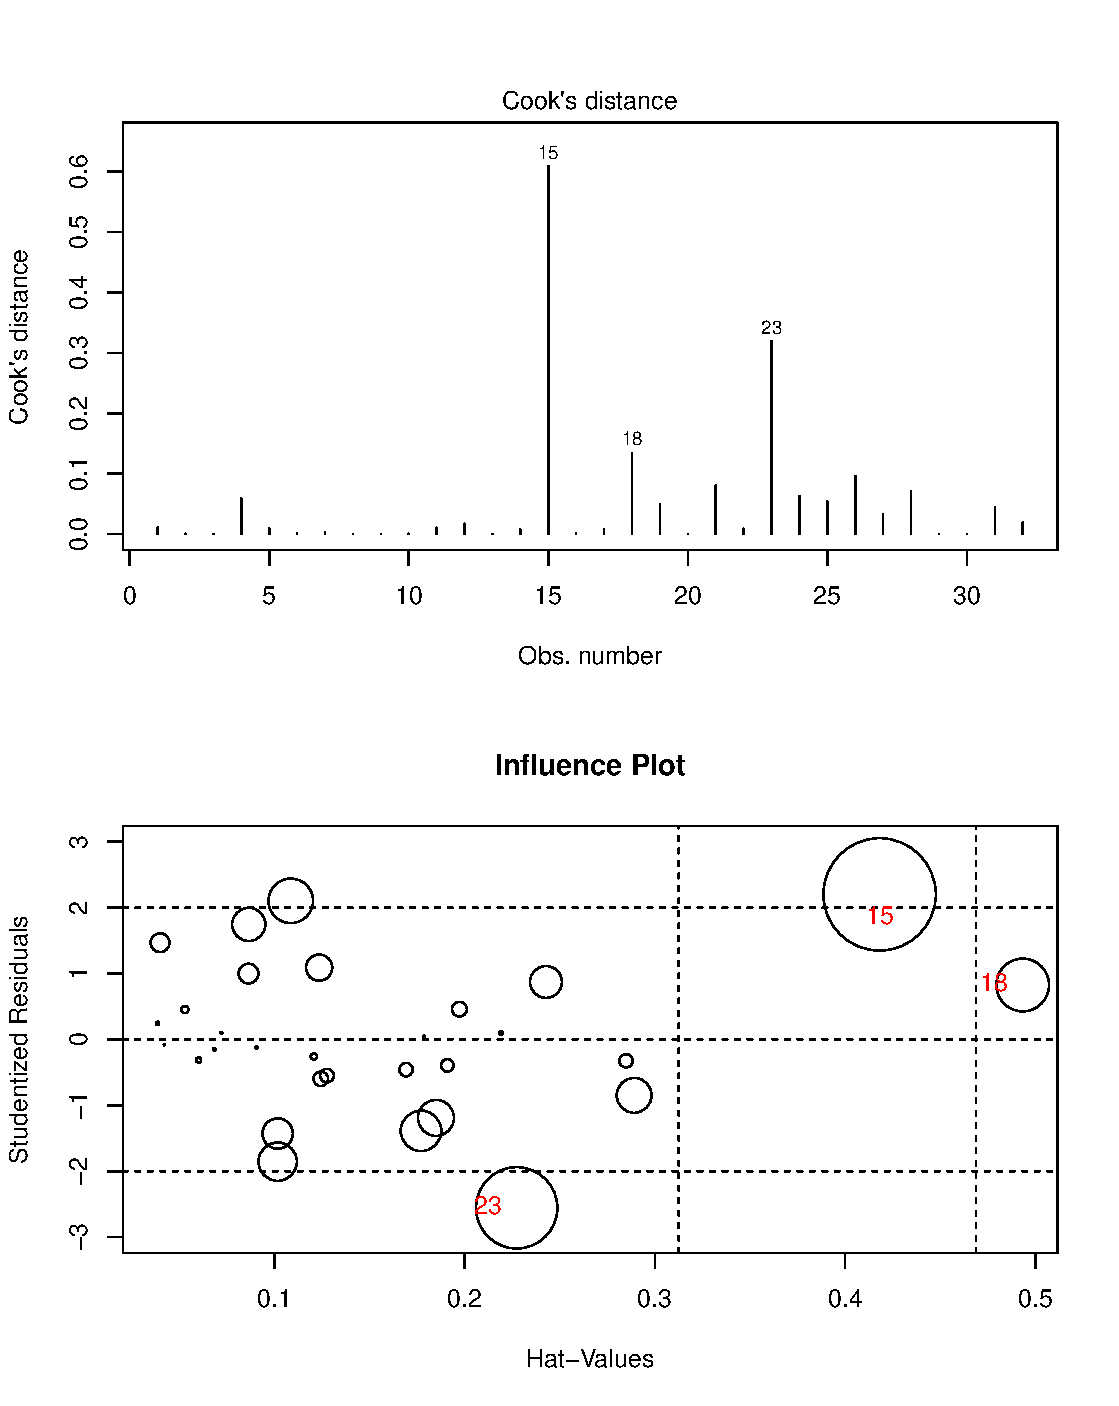
\includegraphics[height=15cm]{plot1}
\end{center}
\caption{The result of Cook's D plot and Influence Plot: Circles in Influence Plot are proportional to Cook's distance\label{inflplot}}
\end{figure}	
	\end{itemize}		
\end{enumerate}

\newpage
\begin{center} \section*{Linear Models in Statistics: HW#5} \end{center}
\textbf{201060072: Boncho Ku}
\begin{enumerate}
   \item[12.19] Redo Example 11.4 with the reparameterization
   \begin{eqnarray*}
   \pmb{\upgamma}=
   \begin{pmatrix}[r]
   \mu+\tau_{1} \\
   \tau_{1}-\tau_{2}
   \end{pmatrix}
   \end{eqnarray*}
   Find $\mathbf{Z}$ and $\mathbf{U}$ by inspection and show that $\mathbf{ZU}=\mathbf{X}$. Then show that 
   $\mathbf{Z}$ can be obtained as $\mathbf{Z}=\mathbf{XU}^{T}(\mathbf{UU}^{T})^{-1}$.
   \begin{itemize}
    \item[Sol.] Let $\mu_{i}=\mu+\tau_{i}$. Then $\mu+\tau_{1}=\mu_{1}$ and $\tau_{1}-\tau_{2}=\mu_{1}-\mu_{2}$. 
    Therefore, design matrix for $\pmb{\upgamma}$, $\mathbf{Z}$ can be written as
    \begin{eqnarray*}
     \mathbf{Z}=
     \begin{pmatrix}[r]
     1 & 0 \\
     1 & 0 \\
     1 & -1 \\
     1 & -1 
     \end{pmatrix}
    \end{eqnarray*} 
    Since $\pmb{\upgamma}=\mathbf{U}\pmb{\upbeta}$, 
     	\begin{eqnarray*}
     	 \pmb{\upgamma} &=&
     	 \begin{pmatrix}[r]
     	  1 & 1 &  0 \\
     	  0 & 1 & -1 
     	 \end{pmatrix}
     	 \begin{pmatrix}[r]
     	 \mu \\
     	 \tau_{1} \\
     	 \tau_{2} 
     	 \end{pmatrix}=
     	 \mathbf{U}\pmb{\upbeta},~~~
     	 \mathbf{U}= 
      	 \begin{pmatrix}[r]
     	  1 & 1 &  0 \\
     	  0 & 1 & -1 
     	 \end{pmatrix}\\     	 
     	 \therefore \mathbf{ZU} &=&
     	 \begin{pmatrix}[r]
	     	1 & 0 \\
	     	1 & 0 \\
	     	1 & -1 \\
	     	1 & -1      	 
     	 \end{pmatrix}
     	 \begin{pmatrix}[r]
      	  1 & 1 &  0 \\
     	  0 & 1 & -1     	 
     	 \end{pmatrix}=
     	 \begin{pmatrix}[r]
     	 1 & 1 & 0 \\
     	 1 & 1 & 0 \\
     	 1 & 0 & 1 \\
     	 1 & 0 & 1 
     	 \end{pmatrix}=\mathbf{X}    	 
     	\end{eqnarray*}
     	Consequently, $\mathbf{Z}$ can be obtained from the equation $\mathbf{Z}=\mathbf{XU}^{T}(\mathbf{UU}^{T})^{-1}$. Therefore, 
     	\begin{eqnarray*}
     	 \mathbf{U}\mathbf{U}^{T}&=&
     	 \begin{pmatrix}[r]
     	 2 & 1 \\
     	 1 & 2 
     	 \end{pmatrix}\\
     	 \mathbf{Z}&=&
     	 \begin{pmatrix}[r]
     	  1 & 1 & 0 \\
     	  1 & 1 & 0 \\
     	  1 & 0 & 1 \\
     	  1 & 0 & 1  	  
     	 \end{pmatrix}
     	 \begin{pmatrix}[r]
     	 1 &  0 \\
     	 1 &  1 \\
     	 0 & -1
     	 \end{pmatrix}
     	 \begin{pmatrix}[r]
     	 2/3 & -1 \\
     	 -1 & 2/3      	 
     	 \end{pmatrix}=
     	 \begin{pmatrix}[r]
		    1 &  0 \\
		    1 &  0 \\
		    1 & -1 \\
		    1 & -1    	 
     	 \end{pmatrix}
     	\end{eqnarray*}
   \end{itemize}
   \item[12.27] Consider the model $y_{ijk}=\mu+\alpha_{i}+\beta_{j}+\gamma_{k}+\epsilon_{ijk},
   ~~i=1,2,~~,j=1,2,~~k=1,2.$
	   \begin{itemize}
	   \item[(a)] Write $\mathbf{X}^{T}\mathbf{X},~\mathbf{X}^{T}\mathbf{y}$, and the normal equation.
	      \begin{itemize}
		    \item[Sol.] The given model is for the $2^{3}$ factorial design and the design matrix can be written as		    
		    \begin{eqnarray*}
		    \mathbf{X}&=&
		    \begin{pmatrix}[r]
			    1 &   1 &   0 &   1 &   0 &   1 &   0 \\
			    1 &   1 &   0 &   1 &   0 &   0 &   1 \\ 
			    1 &   1 &   0 &   0 &   1 &   1 &   0 \\
			    1 &   1 &   0 &   0 &   1 &   0 &   1 \\
			    1 &   0 &   1 &   1 &   0 &   1 &   0 \\
			    1 &   0 &   1 &   1 &   0 &   0 &   1 \\
			    1 &   0 &   1 &   0 &   1 &   1 &   0 \\
			    1 &   0 &   1 &   0 &   1 &   0 &   1
			\end{pmatrix},~~
			\mathbf{X}^{T}\mathbf{X}=
			\begin{pmatrix}[r]
			    8 &   4 &   4 &   4 &   4 &   4 &   4 \\
			    4 &   4 &   0 &   2 &   2 &   2 &   2 \\
			    4 &   0 &   4 &   2 &   2 &   2 &   2 \\
			    4 &   2 &   2 &   4 &   0 &   2 &   2 \\
			    4 &   2 &   2 &   0 &   4 &   2 &   2 \\
			    4 &   2 &   2 &   2 &   2 &   4 &   0 \\
			    4 &   2 &   2 &   2 &   2 &   0 &   4
			\end{pmatrix} \\			
			\mathbf{X}^{T}\mathbf{y} &=&
			\begin{pmatrix}[r]
			    1 &   1 &   1 &   1 &   1 &   1 &   1 &   1 \\
			    1 &   1 &   1 &   1 &   0 &   0 &   0 &   0 \\
			    0 &   0 &   0 &   0 &   1 &   1 &   1 &   1 \\
			    1 &   1 &   0 &   0 &   1 &   1 &   0 &   0 \\
			    0 &   0 &   1 &   1 &   0 &   0 &   1 &   1 \\
			    1 &   0 &   1 &   0 &   1 &   0 &   1 &   0 \\
			    0 &   1 &   0 &   1 &   0 &   1 &   0 &   1
			\end{pmatrix}
			\begin{pmatrix}
			y_{111} \\
			y_{112} \\
			y_{121} \\
			y_{122} \\
			y_{211} \\
			y_{212} \\
			y_{221} \\
			y_{222} 
			\end{pmatrix}=
			\begin{pmatrix}[r]
			y_{...} \\
			y_{1..} \\
			y_{2..} \\
			y_{.1.} \\
			y_{.2.} \\
			y_{..1} \\
			y_{..2} 			
			\end{pmatrix}									 		     
		    \end{eqnarray*}
		    The normal equation can be expressed as
		    \begin{eqnarray*}
			\begin{pmatrix}[r]
			    8 &   4 &   4 &   4 &   4 &   4 &   4 \\
			    4 &   4 &   0 &   2 &   2 &   2 &   2 \\
			    4 &   0 &   4 &   2 &   2 &   2 &   2 \\
			    4 &   2 &   2 &   4 &   0 &   2 &   2 \\
			    4 &   2 &   2 &   0 &   4 &   2 &   2 \\
			    4 &   2 &   2 &   2 &   2 &   4 &   0 \\
			    4 &   2 &   2 &   2 &   2 &   0 &   4
			\end{pmatrix}
			\begin{pmatrix}
			\hat{\mu} \\
			\hat{\alpha}_{1} \\
			\hat{\alpha}_{2} \\
			\hat{\beta}_{1} \\
			\hat{\beta}_{2} \\
			\hat{\gamma}_{1} \\
			\hat{\gamma}_{2}
			\end{pmatrix} &=&
			\begin{pmatrix}[r]
			y_{...} \\
			y_{1..} \\
			y_{2..} \\
			y_{.1.} \\
			y_{.2.} \\
			y_{..1} \\
			y_{..2} 			
			\end{pmatrix}									 					    
		    \end{eqnarray*}
   		  \end{itemize}	    
	   \item[(b)] Find a set of linearly independent estimable functions.
	      \begin{itemize}
		    \item[Sol.] Since $\mathrm{rank}(\mathbf{X})=4$, there exist 4 linearly independent estimable 
		    functions found by reduced row echelon form of $\mathbf{X}$, 
		    \begin{eqnarray*}
		    \mathbf{X}&\sim&
		    \begin{pmatrix}[r]
		    1 &  1 &  0 & 1 &  0 &  1 &  0 \\
		    0 &  0 &  0 & 0 &  0 &  1 & -1 \\
		    0 &  0 &  0 & 1 & -1 &  0 &  0 \\
		    0 &  0 &  0 & 0 &  0 &  0 &  0 \\
		    0 &  1 & -1 & 0 &  0 &  0 &  0 \\
		    0 &  0 &  0 & 0 &  0 &  0 &  0 \\
		    0 &  0 &  0 & 0 &  0 &  0 &  0 \\
		    0 &  0 &  0 & 0 &  0 &  0 &  0 
		    \end{pmatrix}
		    \end{eqnarray*}
		    Therefore, esitmable functions are given by
		    \begin{eqnarray*}
		    \mu+\alpha_{1}+\beta_{1}+\gamma_{1},~\alpha_{1}-\alpha_{2},
		    ~\beta_{1}-\beta_{2},~\gamma_{1}-\gamma_{2}		    
		    \end{eqnarray*}
   		  \end{itemize}	    	   
	   \item[(c)] Define appropriate side conditions and find the resulting solution to the normal equation.	   
	      \begin{itemize}
		    \item[Sol.] Side conditions for the given model are
		    \begin{eqnarray*}
		    \sum_{i=1}^{2}\alpha_{i}=0,~\sum_{j=1}^{2}\beta_{j}=0,~\sum_{k=1}^{2}\gamma_{k}=0
		    \end{eqnarray*}
		    Then a set of non-estimable function is defined by
		    \begin{eqnarray*}
		    \mathbf{T}\pmb{\upbeta}&=&
		    \begin{pmatrix}
		    0 & 1 & 1 & 0 & 0 & 0 & 0 \\
		    0 & 0 & 0 & 1 & 1 & 0 & 0 \\
		    0 & 0 & 0 & 0 & 0 & 1 & 1 
		    \end{pmatrix}\pmb{\upbeta}=0
		    \end{eqnarray*}
		    \begin{eqnarray*}
		     \mathbf{T}^{T}\mathbf{T}=
		      \begin{pmatrix}[r]
			    0 &   0 &   0 &   0 &   0 &   0 &   0 \\
			    0 &   1 &   1 &   0 &   0 &   0 &   0 \\
			    0 &   1 &   1 &   0 &   0 &   0 &   0 \\
			    0 &   0 &   0 &   1 &   1 &   0 &   0 \\
			    0 &   0 &   0 &   1 &   1 &   0 &   0 \\
			    0 &   0 &   0 &   0 &   0 &   1 &   1 \\
			    0 &   0 &   0 &   0 &   0 &   1 &   1		      
		      \end{pmatrix},~~
		      (\mathbf{X}^{T}\mathbf{X}+\mathbf{T}^{T}\mathbf{T})=
		      \begin{pmatrix}[r]
			    8 &   4 &   4 &   4 &   4 &   4 &   4 \\
			    4 &   5 &   1 &   2 &   2 &   2 &   2 \\
			    4 &   1 &   5 &   2 &   2 &   2 &   2 \\
			    4 &   2 &   2 &   5 &   1 &   2 &   2 \\
			    4 &   2 &   2 &   1 &   5 &   2 &   2 \\
			    4 &   2 &   2 &   2 &   2 &   5 &   1 \\
			    4 &   2 &   2 &   2 &   2 &   1 &   5		      
		      \end{pmatrix}
		    \end{eqnarray*}
		    \begin{eqnarray*}
		    (\mathbf{X}^{T}\mathbf{X}+\mathbf{T}^{T}\mathbf{T})^{-1}=
		    \begin{pmatrix}[r]
			  28/32 & -1/4 & -1/4 & -1/4 & -1/4 & -1/4 & -1/4 \\
			   -1/4 &  3/8 &  1/8 &    0 &    0 &    0 & 0 \\
			   -1/4 &  1/8 &  3/8 &    0 &    0 &    0 & 0 \\
			   -1/4 &    0 &    0 &  3/8 &  1/8 &    0 & 0 \\
			   -1/4 &    0 &    0 &  1/8 &  3/8 &    0 & 0 \\
			   -1/4 &    0 &    0 &    0 &    0 &  3/8 & 1/8 \\
			   -1/4 &    0 &    0 &    0 &    0 &  1/8 & 3/8
			 \end{pmatrix}		    
		    \end{eqnarray*}
		    \begin{eqnarray*}
		     \hat{\mu}&=&\frac{28}{32}y_{...}-\frac{24}{32}y_{...}=\frac{1}{8}y_{...}=\bar{y}_{...},\\
		     \hat{\alpha}_{1}&=&-\frac{1}{4}y_{...}+\frac{3}{8}y_{1..}+\frac{1}{8}y_{2..}
		     =\frac{1}{4}y_{1..}-\frac{1}{8}y_{...}=\bar{y}_{1..}-\bar{y}_{...},\\
		     \hat{\alpha}_{2}&=&-\frac{1}{4}y_{...}+\frac{1}{8}y_{1..}+\frac{3}{8}y_{2..}
		     =\frac{1}{4}y_{2..}-\frac{1}{8}y_{...}=\bar{y}_{2..}-\bar{y}_{...},\\
		     \hat{\beta}_{1}&=&\bar{y}_{.1.}-\bar{y}_{...},
		     ~~\hat{\beta}_{2}=\bar{y}_{.2.}-\bar{y}_{...},\\
		     \hat{\gamma}_{1}&=&\bar{y}_{..1}-\bar{y}_{...},
		     ~~\hat{\gamma}_{2}=\bar{y}_{..2}-\bar{y}_{...}\\		    		     
		    \end{eqnarray*}
   		  \end{itemize}	    	    
	   \item[(d)] Show that $H_{0}:\alpha_{1}=\alpha_{2}$ is testable. 
	   Find $\hat{\pmb{\upbeta}}\mathbf{X}^{T}\mathbf{y}=\mathrm{SS}(\mu,\alpha,\beta,\gamma)$ and 
	   $\hat{\pmb{\upbeta}}_{2}\mathbf{X}^{T}_{2}\mathbf{y}=\mathrm{SS}(\mu,\beta,\gamma)$.
	      \begin{itemize}
		    \item[Sol.] Since $\alpha_{1}-\alpha_{2}$ is a linearly independent estimable function 
		    $\pmb{\lambda}^{T}\pmb{\upbeta}$, $H_{0}:\alpha_{1}-\alpha_{2}=0$ is testable, 
		    where $\pmb{\lambda}^{T}=(0,1,-1,0,0,0,0)$. Then,
		    \begin{eqnarray*}
		     \mathrm{SS}(\mu,\alpha,\beta,\gamma)&=&\hat{\pmb{\upbeta}}^{T}\mathbf{X}^{T}\mathbf{y}=
		     \begin{pmatrix}[r]
		     \hat{\mu} & \hat{\alpha}_{1} &\ldots &\hat{\gamma}_{2}\\
		     \end{pmatrix}
		     \begin{pmatrix}[r]
				y_{...} \\
				y_{1..} \\
				y_{2..} \\
				y_{.1.} \\
				y_{.2.} \\
				y_{..1} \\
				y_{..2} 					     
		     \end{pmatrix}\\
		     &=&\hat{\mu}y_{...}+\hat{\alpha}_{1}y_{1..}+\hat{\alpha}_{2}y_{2..}+
		     \hat{\beta}_{1}y_{.1.}+\hat{\beta}_{2}y_{.2.}+\hat{\gamma}_{1}y_{..1}+\hat{\gamma}_{2}y_{..2}\\
		     &=&\frac{1}{8}y_{...}^{2}+\big [\sum_{i=1}^{2}\frac{1}{4}y_{i..}^{2}-\frac{1}{8}y_{...}^{2} \big]
		        +\big [\sum_{j=1}^{2}\frac{1}{4}y_{.j.}^{2}-\frac{1}{8}y_{...}^{2} \big]
		        +\big [\sum_{k=1}^{2}\frac{1}{4}y_{..k}^{2}-\frac{1}{8}y_{...}^{2} \big]\\
		     &=& \mathrm{SS}(\mu)+\mathrm{SS}(\alpha)+\mathrm{SS}(\beta)+\mathrm{SS}(\gamma)\\
		     \mathrm{SS}(\mu,\beta,\gamma)&=& \mathrm{SS}(\mu)+\mathrm{SS}(\beta)+\mathrm{SS}(\gamma)\\
		    \end{eqnarray*}
   		  \end{itemize}	    	   
	   \item[(e)] Construct an analysis of variance table for the test of $H_{0}:\alpha_{1}=\alpha_{2}$.
	      \begin{itemize}
		    \item[Sol.] ANOVA table for testing $H_{0}:\alpha_{1}=\alpha_{2}$ %$\mathrm{SSE}=\sum_{ijk}y_{ijk}^{2}-\mathrm{SS}(\mu,\alpha,\beta,\gamma)$
		  	\begin{table}[ht]
				\begin{center}
				\begin{tabular}{ccccc}
				  \hline
				 Source & Df & Sum Sq & Mean Sq & F value \\ 
				  \hline
				 $\mathrm{SS}(\alpha|\mu,\beta,\gamma)$ & 1 
				 & $\mathrm{SS}(\mu,\alpha,\beta,\gamma)-\mathrm{SS}(\mu,\beta,\gamma)=\mathrm{SS}(\alpha)$ 
				 & $\mathrm{SS}(\alpha)$ & $\mathrm{SS}(\alpha)/\mathrm{MSE}$  \\ 
				Error & 8-4=4 & $\mathrm{SSE}=\sum_{ijk}y_{ijk}^{2}-\mathrm{SS}(\mu,\alpha,\beta,\gamma)$
				& $\mathrm{SSE}/4$ &   \\ 
				\hline
				\end{tabular}
			\end{center}
			\end{table}						    
   		  \end{itemize}	    	   
	   \end{itemize}	   
   \item[13.28] Blood sugar levels were measured on 10 animals from each of five breeds (Daniel 1974, p. 197).
   The results are in Table \ref{bloodtbl}.
   	\begin{itemize}
	    \item[(a)] Test the hypothesis of equality of means for the five bleeds.
	      \begin{itemize}
		    \item[Sol.] Performing one-way ANOVA analysis
% latex table generated in R 2.14.1 by xtable 1.7-0 package
% Sun Jun 10 20:32:44 2012
\begin{table}[ht]
\begin{center}
\begin{tabular}{lrrrrr}
  \hline
 & Df & Sum Sq & Mean Sq & F value & Pr($>$F) \\ 
  \hline
Breed & 4 & 3213.48 & 803.37 & 6.59 & 0.0003 \\ 
  Residuals & 45 & 5485.40 & 121.90 &  &  \\ 
   \hline
\end{tabular}
\caption{ANOVA table for testing equal means for the five breeds}
\end{center}
\end{table}   		  \end{itemize}	    	    
	    \item[(b)] Make the followng four comparisons by means of orthogonal contrasts:	    	    
	    \begin{equation*}
	    \mathrm{A,~B,~C~vs.~D,~E};~~~\mathrm{A,~B~vs.~C};~~~\mathrm{A,~vs.~B};~~~\mathrm{D,~vs.~E};
	    \end{equation*}
	      \begin{itemize}
		    \item[Sol.] The hypothesis for testing the given comparisons can be expressed as $H_{0}:\mathbf{C}
		    \pmb{\upbeta}=0$. The orthogonal contrasts can be expressed as 
		    $$
		    \frac{\mu_{A}+\mu_{B}+\mu_{C}}{3}=\frac{\mu_{D}+\mu_{E}}{2};~~\frac{\mu_{A}+\mu_{B}}{2}=\mu_{C};
		    ~~\mu_{A}=\mu_{B};~~\mu_{D}=\mu_{E}
		    $$
		    $$
		    \mathbf{C}=
		    \begin{pmatrix}[r] 
			    2 &   2 &   2  &  -3 &  -3 \\
			    1 &   1 &  -2  &   0 &   0 \\
			    1 &  -1 &   0  &   0 &   0 \\
			    0 &   0 &   0  &   1 &  -1
			\end{pmatrix}		    
		    $$		   
% latex table generated in R 2.14.1 by xtable 1.7-0 package
% Sun Jun 10 20:32:44 2012
\begin{table}[ht]
\begin{center}
\begin{tabular}{lrrrrr}
  \hline
 & Df & Sum Sq & Mean Sq & F value & Pr($>$F) \\ 
  \hline
Breed                  & 4 & 3213.48 & 803.37 & 6.59 & 0.0003 \\ 
    Breed: A,B,C vs. D,E & 1 & 82.16 & 82.16 & 0.67 & 0.4160 \\ 
    Breed: A,B vs. C     & 1 & 1025.07 & 1025.07 & 8.41 & 0.0058 \\ 
    Breed: A vs. B       & 1 & 5.00 & 5.00 & 0.04 & 0.8404 \\ 
    Breed: D vs. E       & 1 & 2101.25 & 2101.25 & 17.24 & 0.0001 \\ 
  Residuals              & 45 & 5485.40 & 121.90 &  &  \\ 
   \hline
\end{tabular}
\caption{ANOVA table for the orthogonal contrasts}
\end{center}
\end{table}   		  \end{itemize}	    
		\begin{table}[ht]
		\begin{center}
		\begin{tabular}{ccccc}
		  \hline
		  \multicolumn{5}{c}{Breed}\\
		  A & B & C & D & E\\ 
		  \hline
		  124 & 111 & 117 & 104 & 142 \\ 
		  116 & 101 & 142 & 128 & 139 \\
		  101 & 130 & 121 & 130 & 133 \\
		  118 & 108 & 123 & 103 & 120 \\
		  118 & 127 & 121 & 121 & 127 \\
		  120 & 129 & 148 & 119 & 149 \\
		  110 & 122 & 141 & 106 & 150 \\
		  127 & 103 & 122 & 107 & 149 \\
		  106 & 122 & 139 & 107 & 120 \\
		  130 & 127 & 125 & 115 & 116 \\
		  \hline
		\end{tabular}
		\caption{Blood Sugar Levels $(\mathrm{mg}/100\mathrm{g})$ for Ten Animals from Each of Five Breeds\label{bloodtbl}}
		\end{center}
		\end{table}
	 \end{itemize}
	 
   \item[13.33] Weight gains in pigs subjected to four different treatments are given in Table \ref{pigtbl} (Crapmton 
   and Hopkins 1934).
   	\begin{itemize}
   	 \item[(a)] Test the hypothesis of equal mean treatment effects.
	      \begin{itemize}
		    \item[Sol.] One-way ANOVA table without contrasts
% latex table generated in R 2.14.1 by xtable 1.7-0 package
% Sun Jun 10 20:32:44 2012
\begin{table}[ht]
\begin{center}
\begin{tabular}{lrrrrr}
  \hline
 & Df & Sum Sq & Mean Sq & F value & Pr($>$F) \\ 
  \hline
Trt & 3 & 3394.47 & 1131.49 & 6.57 & 0.0012 \\ 
  Residuals & 36 & 6197.90 & 172.16 &  &  \\ 
   \hline
\end{tabular}
\caption{ANOVA table for testing equal means for the four treatments}
\end{center}
\end{table}   		  \end{itemize}	       	 
   	 \item[(b)] Using contrasts, compare treatments 1, 2, 3 vs. 4; 1, 2, vs. 3; and 1 vs. 2.
	      \begin{itemize}
		    \item[Sol.] Contrast matrix for the given comparison
		    \begin{eqnarray*}
		    \mathbf{C}&=&
		    \begin{pmatrix}[r]
		     1  &  1  &  1 &  -3 \\
    		 1  &  1  & -2 &   0 \\
    		 1  & -1  &  0 &   0		    
		    \end{pmatrix}
		    \end{eqnarray*}
% latex table generated in R 2.14.1 by xtable 1.7-0 package
% Sun Jun 10 20:32:44 2012
\begin{table}[ht]
\begin{center}
\begin{tabular}{lrrrrr}
  \hline
 & Df & Sum Sq & Mean Sq & F value & Pr($>$F) \\ 
  \hline
Trt                & 3 & 3394.47 & 1131.49 & 6.57 & 0.0012 \\ 
    Trt: 1,2,3 vs. 4 & 1 & 1944.07 & 1944.07 & 11.29 & 0.0019 \\ 
    Trt: 1,2 vs. 3   & 1 & 72.60 & 72.60 & 0.42 & 0.5202 \\ 
    Trt: 1 vs. 2     & 1 & 1377.80 & 1377.80 & 8.00 & 0.0076 \\ 
  Residuals          & 36 & 6197.90 & 172.16 &  &  \\ 
   \hline
\end{tabular}
\caption{ANOVA table for the orthogonal contrasts}
\end{center}
\end{table}   		  \end{itemize}	       	 
 		\begin{table}[ht]
		\begin{center}
		\begin{tabular}{cccc}
		\hline 
		\multicolumn{4}{c}{Treatment}\\
		1 & 2 & 3 & 4 \\
		\hline
		165 & 168 & 164 & 185 \\		
		159 & 180 & 156 & 195 \\
		159 & 180 & 189 & 186 \\
		167 & 166 & 138 & 201 \\
		170 & 170 & 153 & 165 \\
		146 & 161 & 190 & 175 \\
		130 & 171 & 160 & 187 \\
		151 & 169 & 172 & 177 \\
		164 & 179 & 142 & 166 \\
		158 & 191 & 155 & 165 \\
		\hline
		\end{tabular}
		\caption{Weight Gain of Pigs Subjected to Four Treatments\label{pigtbl}}
		\end{center}
		\end{table}  	 
   	\end{itemize}
\end{enumerate}
\end{document}

